% -*-memoria.tex-*-
% Este fichero es parte de la plantilla LaTeX para
% la realización de Proyectos Final de Carrera, protegido
% bajo los términos de la licencia GFDL.
% Para más información, la licencia completa viene incluida en el
% fichero fdl-1.3.tex

% Copyright (C) 2009 Pablo Recio Quijano 

%-------------------------------------------------------
% ---- Plantilla para libros / memorias PFC -----

% Realizada por Pablo Recio Quijano y Noelia Sales Montes 
% Formato de portada y primera página tomado del PFC de
% Francisco Javier Vázquez Púa, en su proyecto 'libgann'
% -------------------------------------------------------

\documentclass[spanish,a4paper,11pt]{book}


\usepackage{./estilos/estiloBase} % Básicamente son todas las
                                  % librerias usadas. En caso de que
                                  % falten librerias se van añadiendo
                                  % al fichero.
\usepackage{./estilos/colores}  % Algunos colores ya generados, para
                                % los algunos estilos más avanzados.
\usepackage{./estilos/comandos} % Algunos comandos personalizados

\graphicspath{{./imagenes/}} % Indicamos la ruta donde se encuentran
                             % las imagenes, para ahorrarnos la ruta
                             % completa, y solo modificar aquí si en
                             % un momento dado lo movemos

\bibliography{references}

\begin{document}

% Renombramos las figuras y las tablas
\renewcommand{\figurename}{Figura}
\renewcommand{\listfigurename}{Indice de figuras}
\renewcommand{\tablename}{Tabla}
\renewcommand{\listtablename}{Indice de tablas}

\pagestyle{empty}
% -*-portada.tex-*-
% Este fichero es parte de la plantilla LaTeX para
% la realización de Proyectos Final de Carrera, protejido
% bajo los términos de la licencia GFDL.
% Para más información, la licencia completa viene incluida en el
% fichero fdl-1.3.tex

% Fuente tomada del PFC 'libgann' de Javier Vázquez Púa

\begin{titlepage}

  \begin{center}

    
\includegraphics[scale=0.2]{logo_uca.png} \\
    
    \vspace{2.0cm}
    
    \LARGE{\textbf{ESCUELA SUPERIOR DE INGENIERÍA}} \\
    
    \vspace{1.0cm}
    
    \Large{\textbf{GRADO EN INGENIERÍA INFORMÁTICA}} \\
    
    \vspace{3.0cm}
    
    \Large{PROYECTO DE APP DE RECOGIDA DE ENSERES} \\
    
    \vspace{2.0cm}
    
    \Large{Diego Rubio Abujas} \\
  
    \vspace{0.5cm}

    \large{\today}
    
  \end{center}
\end{titlepage}

\cleardoublepage

% -*-primerahoja.tex-*-
% Este fichero es parte de la plantilla LaTeX para
% la realización de Proyectos Final de Carrera, protejido
% bajo los términos de la licencia GFDL.
% Para más información, la licencia completa viene incluida en el
% fichero fdl-1.3.tex

% Fuente tomada del PFC 'libgann' de Javier Vázquez Púa

\begin{center}

  
\includegraphics[scale=0.2]{logo_uca.png} \\

  \vspace{2.0cm}

  \Large{ESCUELA SUPERIOR DE INGENIERÍA} \\

  \vspace{1.0cm}

  \large{GRADO EN INGENIERÍA INFORMÁTICA} \\

  \vspace{2.0cm}

  \large{PROYECTO DE APP DE RECOGIDA DE ENSERES} \\

  \vspace{1.0cm}

\end{center}

\begin{itemize}
\item \large{Departamento: Lenguajes y sistemas informáticos}
\item \large{Director del proyecto: Lorena Gutierrez Madroñal}
\item \large{Autor del proyecto: Diego Rubio Abujas}
\end{itemize}

\vspace{1.0cm}

\begin{flushright}
  \large{Cádiz, \today} \\

  \vspace{2.5cm}

  \large{Fdo: Diego Rubio Abujas}
\end{flushright}

\cleardoublepage
\pagestyle{plain}

\frontmatter % Introducción, índices ...

% -*-previo.tex-*-
% Este fichero es parte de la plantilla LaTeX para
% la realización de Proyectos Final de Carrera, protejido
% bajo los términos de la licencia GFDL.
% Para más información, la licencia completa viene incluida en el
% fichero fdl-1.3.tex

% Copyright (C) 2009 Pablo Recio Quijano 

\section*{Agradecimientos}

Me gustaria agradecer y/o dedicar este texto a ...

\cleardoublepage

\section*{Licencia} % Por ejemplo GFDL, aunque puede ser cualquiera

Este documento ha sido liberado bajo Licencia GFDL 1.3 (GNU Free
Documentation License). Se incluyen los términos de la licencia en
inglés al final del mismo.\\

Copyright (c) 2009 Pablo Recio Quijano.\\

Permission is granted to copy, distribute and/or modify this document under the
terms of the GNU Free Documentation License, Version 1.3 or any later version
published by the Free Software Foundation; with no Invariant Sections, no
Front-Cover Texts, and no Back-Cover Texts. A copy of the license is included in
the section entitled "GNU Free Documentation License".\\

\cleardoublepage

\section*{Notación y formato}

Aquí incluiremos los aspectos relevantes a la notación y el formato a
lo largo del documento. Para simplificar podemos generar comandos
nuevos que nos ayuden a ello, ver \texttt{comandos.sty} para más
información. 

Cuando nos refiramos a un programa en concreto, utilizaremos la
notación: \\ \programa{emacs}.\\

Cuando nos refiramos a un comando, o función de un lenguaje, usaremos
la notación: \\ \comando{quicksort}.\\
\cleardoublepage

\tableofcontents
\listoffigures
\listoftables

\mainmatter % Contenido


% SECCIONES
\chapter{Prolegómeno}
\section{Introducción}
\subsection{Motivación}
	Se pretende dar solución mediante un proyecto informático a una problemática real que actualmente se está solucionando mediante trámites gestionados vía telefónica. Inicialmente se observa un problema cercano localizado en algún organismo público y que pueda ser escalable. La búsqueda de un problema al cuál dar solución se inicia en la localidad en la que reside el autor de este proyecto. \\

Día a día, se puede observar que hay una tendencia creciente al reciclaje tanto de muebles como de electrodomésticos. Según estudios \cite{AndaluciaEcologica:web} llevados a cabo por la Consejería de Medio Ambiente de la Junta de Andalucía: se observa que desde el año 1999 al 2008 se produjo un considerable incremento en la cantidad de Plantas de clasificación, recuperación, transferencia y vertederos de apoyo; por otro lado se redujeron bastante los vertederos de residuos no peligrosos. Todo ello nos lleva a observar una considerable inversión por parte de la comunidad autónoma de Andalucía por el reciclaje. Por otra parte también de dicho estudio se puede sacar la conclusión de que hay un mayor indice generalizado de residuos por habitante tal y como se observa en la gráfica, y que es una tendencia de todas las provincias de la comunidad autónoma de Andalucía. Si revisamos el \textit{Plan Director Territorial de Residuos No Peligrosos}\cite{conserjeria_de_medio_ambiente_junta_de_andalucia_plan_2011} redactado por el Consejo de Gobierno de la Junta de Andalucía en el 2011, en lo referido a la recogida de aparatos eléctricos y electrodomésticos hay un considerable crecimiento en el número de electrodomésticos depositados como residuos, y se prevé una duplicación de dicho demanda en 12 años. Adicionalmente, se indica que el 89\% de ellos proceden de hogares particulares, y destaca el incremento de plantas dedicadas al tratamiento de dichos residuos. Se deja claro que la recogía de dichos enseres será gestionado por cada uno de los ayuntamientos. \\

De todo lo anterior, se puede observar un incremento de puntos limpios y una mayor organización de los residuos depositados. Se puede concluir, que durante los últimos años se ha ido incrementando considerablemente el número de residuos voluminosos depositados en cada uno de los municipios, esto se debe principalmente a la cada vez mayor tendencia a renovación de muebles o electrodomésticos y a la rotura o avería de estos. \\

\begin{figure}[H]
\begin{center}
    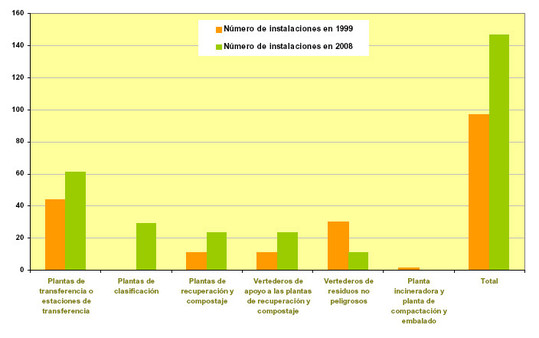
\includegraphics[scale=0.60]{grafica-plantas-residuos.jpg}
\end{center}
    \caption{Infraestructura para la gestión de residuos domiciliarios (1999-2008). Fuente: Borrador Plan Director Territorial de Residuos no peligrosos de Andalucía 2010-2019}
\end{figure}

\begin{figure}[H]
\begin{center}
    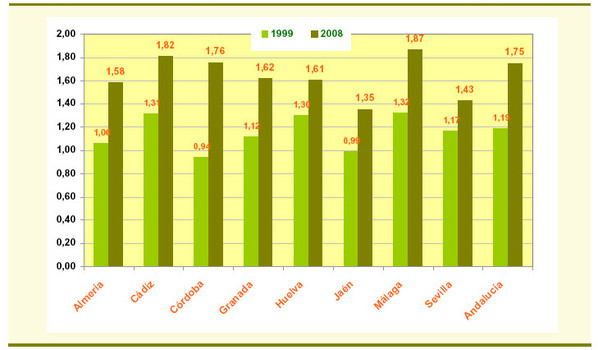
\includegraphics[scale=0.60]{grafica-residuos-habitante.jpg}
\end{center}
    \caption{Evolución de la generación de Residuos Urbanos 1999-2008 (Kg./hab/día). Fuente: Borrador Plan Director Territorial de Residuos no peligrosos de Andalucía 2010-2019}
\end{figure}

La operativa habitual a la hora de gestionar la recogida de dichos residuos es bastante similar en unos u otros municipios. Para informarnos de cómo se suele realizar la tramitación de la recogida de enseres se han consultado empresas municipales de la zona, a continuación se muestra una tabla con la información obtenida. \\

% Tabla de estado actual del servicio de recogida de enseres.
\begin{sidewaystable}
    \centering
\begin{tabular}{|c|l|ll}
\cline{1-2}
\textbf{Localidad}       & \multicolumn{1}{|c|}{\textbf{Operativa}}                                                                                                                    &  \\ \cline{1-2}
Cádiz                    & \begin{tabular}[c]{@{}c@{}}previa petición de los mismos al teléfono 956 262611\\ de lunes a viernes.\end{tabular}                                          &               \\ \cline{1-2}
El Puerto de Santa María & previa petición de los mismos al teléfono 900 102 697                                                                                                       &              \\ \cline{1-2}
Puerto Real              & previa petición de los mismos al teléfono 956474448                                                                                                         &              \\ \cline{1-2}
San Fernando             & \begin{tabular}[c]{@{}c@{}}previa petición de los mismos al teléfono 956 880 884 o bien \\ solicitud web mediante portal web del ayuntamiento.\end{tabular} &              &  \\ \cline{1-2}
Jerez de la frontera     & \begin{tabular}[c]{@{}c@{}}Recogida nocturna por zonas, no requiere petición previa, pero \\  sí informarse de que día se recoge en cada zona al teléfono gratuito 010.\end{tabular} &              \\ \cline{1-2}
\end{tabular}
\caption{Operativas de recogida de enseres de ayuntamientos consultados}
\end{sidewaystable}

Actualmente lo general es ofrecer la realización de dicho servicio de recogida mediante un número de teléfono gratuito puesto a disposición de la ciudadanía. A pesar de ello, hay un cierto desconocimiento por parte de ésta de en qué consiste el servicio y qué trámites hay que llevar a cabo para solicitar la recogida: prueba de ello es que, en el término de Puerto Real sólo el 40\% de las intervenciones de recogida fueron realizadas el año pasado por aviso de los usuarios \cite{articulo:lavozdecadiz}. Se hace necesario tanto promover una mayor cultura de reciclaje, como facilitar y dar una mayor comodidad a los trámites para solicitar la recogida de enseres. Se trata pues de buscar un medio alternativo al número de teléfono gratuito con horario específico de atención al cliente y un único operador tramitando una tras otra peticiones de similar tipología. \\

Inicialmente se barajan dos posibles soluciones, por un lado ofrecer una aplicación web que gestione ese tipo de peticiones y por otro una aplicación para terminales \textit{
smartphone}. Según el informe \textit{The Digitar Consumer} \cite{the_nielsen_company_digital_2014}, se puede observar que cada vez se utilizan más los dispositivos móviles para navegar por internet y realizar diversas gestiones. De media, los usuarios pasan más 34 horas y 17 minutos al mes con su terminal smartphone navegando por internet o utilizando aplicaciones, mientras que haciendo uso del ordenador y realizando esas mismas tareas pasan de media 27 horas y 3 minutos mensuales. Es por ello que para llegar a un mayor número de usuarios, y dada esta tendencia actual, interesa ofrecer la solución al problema planteado mediante la oferta de una alternativa que permita realizar dicha gestión mediante una aplicaciones disponible desde teléfono móvil. \\

De entre las diversas plataformas móviles existente interesará la mayormente usada en España, ya que interesa maximizar la difusión de la aplicación y de esta forma llegar al máximo número de ciudadanos. Durante el mes de febrero del 2014 según un estudio realizado por \textit{Kantar WordPanel} \cite{kantar_wordpanel_publications_2014} se observa que la plataforma de mayor difusión en nuestro país es Android con un 86\% de cuota de mercado. Por lo tanto se opta por ofrecer una funcionalidad rutinaria que a día de hoy se está llevando a cabo vía telefónica hablando con un operador mediante una aplicación móvil para la plataforma de mayor difusión que en este caso es \textit{Android}.\\

\begin{figure}[H]
\begin{center}
    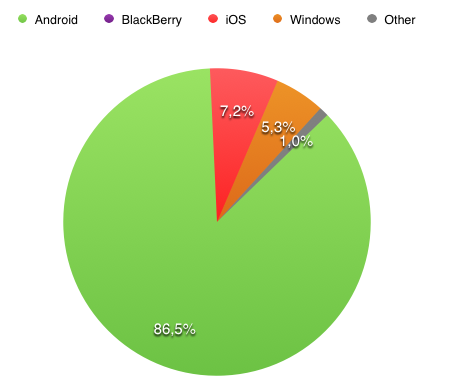
\includegraphics[scale=0.60]{estudio-plataformas.png}
\end{center}
    \caption{Smartphone OS market share España (febrero del 2014)}
\end{figure}

\subsection{Descripción del sistema actual}
	Tras la entrevista llevada a cabo, se procede a describir cómo funciona el sistema actual. Además de la entrevista se ha consultad la web empresarial de Apresa21\cite{apresa21:web}.

% Información del servicio prestado
\subsubsection*{Servicio ofertado}
El servicio proporcionado a habitantes de la localidad de Puerto Real consiste en gestionar la recogida de muebles o electrodomésticos de tamaño considerable, y su posterior traslado al punto limpio. Dicho servicio es gratuito y coree a cargo del ayuntamiento de Puerto Real. Dada la gratuidad tanto del servicio como de un número de teléfono puesto a disposición de la ciudadanía, se limita el número de peticiones diarias por habitante en tres enseres diarios. Para llevar a cabo dicha tarea la empresa \textit{Apresa 21} dispone de un camión que todos los días realiza una ruta planificada en función de los pedidos realizados y que tiene una capacidad para 25 muebles. \\

% Teléfono disponible
\subsubsection*{Teléfono gratuito}
Actualmente para solicitar la recogida de un mueble o electrodoméstico el habitante de la localidad debe ponerse en contacto con número de teléfono gratuito puesto a disposición para dicha finalidad. En dicha llamada, un teleoperador informará al usuario de las características del servicio ofrecido por el ayuntamiento y solicitará al usuario información sobre los objetos que desea que sean recogidas. También se le solicitará algún identificador su nombre, o si es posible su nombre y apellidos. Una vez se ha identificado al usuario también se requerirán su dirección y un número de teléfono. \\

Una vez el usuario ha descrito que desea depositar, el teleoperador consulta las solicitudes que se han realizado anteriormente y concierta un día para la recogida. Se informa al solicitante de la fecha en la que se recogerán sus objetos, la hora a la que deberá depositarlos y el punto en que se efectuará la recogida por parte del camión. Una vez informado al usuario, se finaliza la llamada telefónica y se registra la solicitud. Este procedimiento es el habitual para estos casos, es un sistema mas costoso, poco automatizado, que requiere de más tiempo. Además requiere que aquellos usuarios interesados dispongan del teléfono y efectúan una llamada telefónica en el horario de atención al público. Además. los usuarios tienen la información únicamente cuando realizan la llamada, posteriormente deben recordar la fecha de recogida, el lugar y toda la información explicada por el teleoperador. No existe un soporte físico donde consultar la recogida, las condiciones y las características. \\

En dichas llamadas además de  tener que explicar al ciudadano todo el procedimiento a seguir, hay que explicar determinadas reglas como por ejemplo el hecho de que deban depositar los enseres a partir de una determinada hora de la noche para evitar posible actos vandálicos; la limitación de 3 muebles por día y por persona. \\

% Funcionamiento interno
\subsubsection	*{Ejecución de la operativa}
Se realizan cada día 25 recogías como máximo (Debido a la capacidad del camión), el conductor del camión dispone de una ruta en la que se contemplan todos los puntos de recogida. Cuando el camión llega a un punto pueden darse dos circunstancias: o bien se localizan los enseres en cuyo caso se colocan en el camión y se pasa al siguiente punto, o bien que haya alguna incidencia en el proceso de recogida. De entre las incidencias más comunes se pasan a enumerar y explicar a continuación: \\

% Incidencias
\begin{enumerate}
\item \textbf{Enseres ausentes o en una ubicación inaccesible: }puede ocurrir que al llegar al punto de recogida el conductor del camión no localice los enseres indicados, o bien se encuentren dentro de una casa o casa puerta a la que no responda nadie. En estos casos el conductor se pone en contacto desde su teléfono móvil con la central, y ésta contacta con vía telefónica con el usuario para resolver la incidencia de forma individual.
\item \textbf{Los objetos depositados difieren de la petición realizada: }este hecho ocurre cuando el conductor del camión encuentra que ya sea el número de objetos depositados y/o su casuística difieren de lo solicitado. Este puede deberse a varios motivos:  los vecinos del solicitante han optado por aprovechar la petición de recogida para depositar (sin previo aviso) sus propios muebles, o bien el usuario por algún motivo ha indicado de manera errónea (intencionada o desintencionadamente) el tipo y/o número de enseres que iba a depositar. Cuando este tipo de incidencia ocurre hay que alterar toda la ruta, aumentar el número de viajes, transbordos e incluso puede que haya que modificar la operativa para dicho día.
\end{enumerate}

% Zonas rurales
Aunque se ha indicado que todos los días se recogen 25 enseres, hay una excepción referida a la zonas geográficas calificada como áreas rurales. En dichas zonas la recogida se realiza un único día a la semana dado que tienen menos demanda de servicio y dispone de espacios en los que almacenar los enseres a la espera de ser recogidos. \\

\subsection{Objetivos y alcance del proyecto}
	% Se incluyen todas las tablas de objetivo
% Gestionar solicitudes para recogida de enseres
\begin{table}[H]
\centering
\begin{tabular}{|l|l|}
\hline
\multicolumn{1}{|c|}{\textbf{OBJ-001}} & \textbf{Gestionar solicitudes para recogida de enseres}                                                                                                                                                                                                                                                                                                                                                                                                                                                                                                                                                                                                                                                                                                                                                                        \\ \hline
\textbf{Versión}                       & 1.0 (17/02/2014)                                                                                                                                                                                                                                                                                                                                                                                                                                                                                                                                                                                                                                                                                                                                                                                                         \\ \hline
\textbf{Autor}                         & Diego Rubio Abujas                                                                                                                                                                                                                                                                                                                                                                                                                                                                                                                                                                                                                                                                                                                                                                                                       \\ \hline
\textbf{Fuentes}                       & Epresa21                                                                                                                                                                                                                                                                                                                                                                                                                                                                                                                                                                                                                                                                                                                                                                                                                 \\ \hline
\textbf{Descripción}                   & \textit{\begin{tabular}[c]{@{}c@{}}El sistema deberá gestionar las solicitudes de ciudadanos\\ interesados en que se les lleve a cabo la recogida de enseres\\ para su traslado al punto limpio. Esta recogida se realizará\\ por medio de una aplicación puesta a disposición para su \\ smartphone. Para gestionar la petición inicialmente el \\ solicitante enviará una solicitud con el número y tipo de\\ enseres que desea que le sean recogidos. El sistema dará\\ respuesta a dicha solicitud aceptándola o denegándola.\\ En caso de denegarla indicará el motivo, en caso de \\ aceptarla indicará la fecha, ubicación y explicará el \\ procedimiento que debe llevar a cabo para depositar\\ dichos enseres en la vía pública. Además el sistema \\ registrará todas las peticiones cursadas.\end{tabular}} \\ \hline
\textbf{Importancia}                   & Vital                                                                                                                                                                                                                                                                                                                                                                                                                                                                                                                                                                                                                                                                                                                                                                                                                    \\ \hline
\end{tabular}
\caption{OBJ-001 Gestionar solicitudes para recogida de enseres}
\end{table}

\begin{table}[H]
\centering
\begin{tabular}{|l|l|}
\hline
\multicolumn{1}{|c|}{\textbf{OBJ-002}} & \textbf{Información de reciclaje}                                                                                                                                                                                                                                                                               \\ \hline
\textbf{Versión}                       & 1.0 (17/02/2014)                                                                                                                                                                                                                                                                                                              \\ \hline
\textbf{Autor}                         & Diego Rubio Abujas                                                                                                                                                                                                                                                                                                            \\ \hline
\textbf{Fuentes}                       & Epresa21                                                                                                                                                                                                                                                                                                                      \\ \hline
\textbf{Descripción}                   & \textit{\begin{tabular}[c]{@{}c@{}}El sistema deberá informar a los usuarios\\ acerca de las gestiones que hay que \\ realizar para el reciclaje de los distintos\\ tipos de residuos existentes. Todo ello\\ debe ser en una interfaz amigable,\\ visualmente atractiva y sin excesiva\\ longitud de texto.\end{tabular}} \\ \hline
\textbf{Importancia}                   & Media                                                                                                                                                                                                                                                                                                                         \\ \hline
\end{tabular}
\caption{OBJ-002 Información de reciclaje}
\end{table}

\begin{table}[H]
\centering
\begin{tabular}{|l|l|}
\hline
\multicolumn{1}{|c|}{\textbf{OBJ-003}} & \textbf{Consultar peticiones}                                                                                                                                                                                                 \\ \hline
\textbf{Versión}                       & 1.0 (17/02/2014)                                                                                                                                                                                                              \\ \hline
\textbf{Autor}                         & Diego Rubio Abujas                                                                                                                                                                                                            \\ \hline
\textbf{Fuentes}                       & Epresa21                                                                                                                                                                                                                      \\ \hline
\textbf{Descripción}                   & \textit{\begin{tabular}[c]{@{}c@{}}El sistema deberá mostrar las peticiones\\ realizadas por los usuarios, y permitir generar\\ un informe para planificar la recogida de enseres\\ y elaborar estadísticas.\end{tabular}} \\ \hline
\textbf{Importancia}                   & Media                                                                                                                                                                                                                         \\ \hline
\end{tabular}
\caption{OBJ-003 Consultar peticiones}
\end{table}
\begin{table}[H]
\centering
\begin{tabular}{|l|l|}
\hline
\multicolumn{1}{|c|}{\textbf{OBJ-004}} & \textbf{Mostrar mapa con puntos limpios}                                                                                                                                                 \\ \hline
\textbf{Versión}                       & 1.0 (17/02/2014)                                                                                                                                                                         \\ \hline
\textbf{Autor}                         & Diego Rubio Abujas                                                                                                                                                                       \\ \hline
\textbf{Fuentes}                       & Epresa21                                                                                                                                                                                 \\ \hline
\textbf{Descripción}                   & \textit{\begin{tabular}[c]{@{}c@{}}El sistema deberá mostrar al usuario un mapa \\ de la localidad con los distintos puntos de recogida\\ y puntos limpios disponibles.\end{tabular}} \\ \hline
\textbf{Importancia}                   & Media                                                                                                                                                                                    \\ \hline
\end{tabular}
\caption{OBJ-004 Mostrar mapa con puntos limpios}
\end{table}

\subsection{Organización del documento}
\newpage
\section{Planificación}
\subsection{Metología de desarrollo}
	% ¿Qué son las metodologías ágiles?
Las metodologías ágiles nos permiten una mayor flexibilidad que las metodologías tradicionales de desarrollo, que debido a una mayor rigidez en sus procesos y en la documentación no nos permiten ajustarnos a cambios que pueden producirse en las necesidad del cliente, en el mercado o en desafíos que pueda plantearnos las tecnologías que planeamos emplear. Además exísteme determinadas metodologías probadas y centradas para el desarrollo de aplicaciones móviles. A continuación se procede a explicar en qué consisten las metodologías ágiles y a hablar de la metodología \textit{Mobile-D}, escogida para la realización de dicho proyecto.

\subsubsection*{Metodologías ágiles}
En el año 2001 se celebró una reunión en Utah de la cual surgió el término ``ágil'' aplicado al desarrollo de software. El objetivo de dicha reunión fue establecer principios y valores que permitirían a equipos de desarrollo agilizar y responder a todo los cambios que surgen en los proyectos. Estos "métodos ágiles" se plantean como una alternativa a las metodologías convencionales más rígidas y centradas en la documentación que se genera tras cada actividad. \\

Las motivaciones principales que llevan a estas nuevas metodologías tratan de dar solución a dos problemáticas: por un lado el alto porcentaje de proyectos que fracasan o se retrasan; y por otro la baja calidad de estos\cite{metodologidesarrollo2009}. \\

\subsubsection*{Mobile-D}
% ¿Qué es?
Dentro de las metodologías ágiles, Mobile-D es una creada por el VTT\footnote{Technical Research Centre of Finland} en colaboración estrecha con la industria de TI finlandesas. Se desarrolla en el año 2004 para un proyecto finlandés llamado ICAROS. Esta metodología se crea centrándose en el desarrollo de aplicaciones móviles. Cabe destacar que los autores consideraron dos aspectos: por un lado equipos pequeños de 10 personas o menos, y por otro la disposición de proyectos funcionales en menos de 10 semanas. Todo ello lo hace idóneo para el desarrollo de aplicaciones móviles \cite{metodologidesarrollo2009}. \\
Esta metodología es una mezcla de técnicas utilizadas por otras metodologías ágiles tales como \textit{eXtreme Programming},\textit{Crystal methodologies} y \textit{Rational Unified Process}. De la \textit{eXtreme Programming} se emplean prácticas de desarrollo, \textit{Crystal metodologies} proporciona inputs importantes en lo referidos a escalabilidad de los métodos; y de \textit{Rational Unified Process} se toman las bases para el diseño completo del ciclo de vida. \\
% Fases
Para la planificación de dicha metodología se establecen cinco fases. A excepción de la fase inicial, en cada una de las fases se establece un día de planificación y uno de entrega. Las fases \cite{AgileMobileD} se muestran en el siguiente gráfico:
\begin{figure}[H]
\centering
    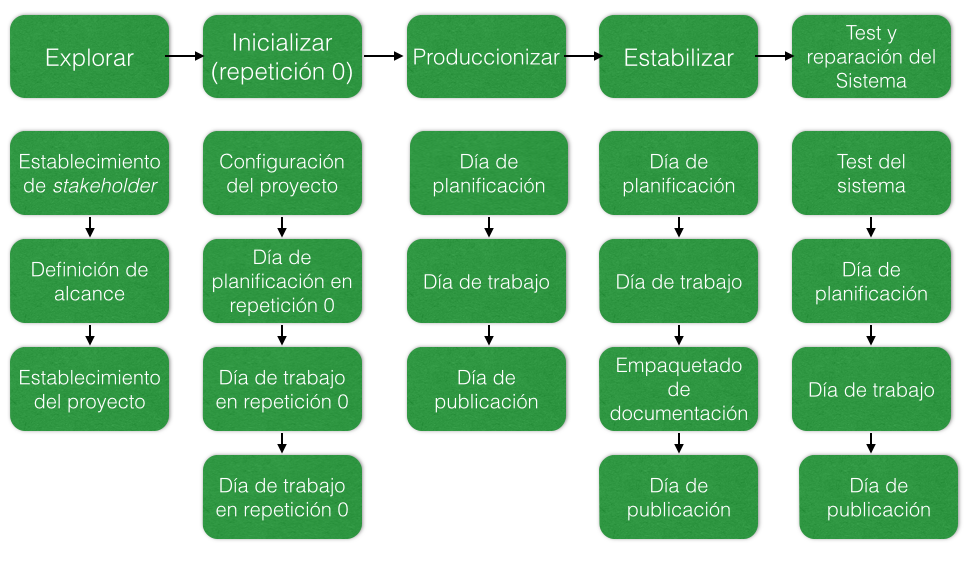
\includegraphics[scale=0.35]{etapasmobile-d.png}
    \caption{Fases de la metodología Mobile-D}
\end{figure}
% Se enumeran las fases de la metodología
\begin{itemize}
    \item \textbf{Exploración: }el propósito de dicha fase es planificar y establecer el inicio del proyecto. Se establecen los \textit{stakeholders}, se definen los objetivos y se lleva a cabo la planificación del proyecto.
    \item \textbf{Inicialización: }se identifican los recursos necesarios, se establece el entorno de desarrollo y la formación inicial.
    \item \textbf{Productización: }en esta fase se realiza una repetición iterativa de subfases. Se emplean técnicas de \textit{test driven development} para el desarrollo.
    \item \textbf{Estabilización: }se procede a la integración de todas las partes del sistema.
    \item \textbf{Test y reparación del sistema: }se prueba el sistema según los requisitos establecidos, se llevan a cabo correcciones y finalmente se obtiene una versión estable y funcional.
\end{itemize}
\subsection{Planificación del proyecto}
	%Define the timeline: is a step where the overall schedule for the project is estimated. There are two starting points for this: 1) Flexible ending (i.e., flexible investments and flexible functionality) and 2) Fixed ending. The latter one is described in the variant section of this pattern. In Agile software development the situation may often be that the finishing time of the project is dependent on the completion of the product (due to the constantly changing/involving requirements). Thus, a clear timeline can not be set but rather estimations.

Inicialmente se define una linea temporal cuya fecha de inicio es la concepción de la idea y la primera entrevista de elicitación de requisitos. La idea del proyecto fue concebida por el autor el día \textit{5 de noviembre del 2013}. Posteriormente la entrevista se realizó el \textit{jueves 21 de noviembre de 2013}. Una vez realizada la entrevista se contactó con la tutora del proyecto, se le expuso la idea y se le hizo entrega de una transcripción de la entrevista; dicho primer encuentro se llevó a cabo \textit{el martes 10 de diciembre de 2013}. \\

Se toma como fecha de inicio la fecha en la cual se comenzó a desarrollar el documento, la formación, definición de objetivos,planificación y desarrollo del proyecto. Por lo tanto se considera como \textbf{fecha de incicio} el día \textit{5 de enero de 2014}. \\
 
%Define the rhythm: is a step where the lengths and number (estimated) of the iterations (i.e., product releases) is set. This also included the identification of other main checkpoints (i.e., milestones) related to, for example, quality assurance issues.
El ritmo de entrega una vez comience el desarrollo se tratará de que sea cada dos semanas. Éstas iteraciones siempre que sea posible serán enviadas para su evaluación al \textit{Auditor Externo}. \\

%Define/estimate the investments: is a step where the interest groups commonly agree on the costs of the project; the effort and financial investments for the product development. However, considering the flexible ending of the project, these investments may be highly dependent on the changes on, for example, requirements. Some decisions, however, need to be established concerning the estimations as well as their possible revision later on.
Aunque en el momento de inicio del proyecto se desconoce la fecha exacta de exposición se ha establecido que se llevará a cabo entre los meses de junio y julio. Por lo que, a efectos de planificación, se impondrá como \textbf{fecha de finalización} del proyecto el día \textit{1 de junio de 2014}. Esta fecha de final tiene cierta flexibilidad, dado en cuanto se conozca la fecha exacta de exposición del pfg se podrá modificar la planificación en función de ello. \\

En la etapa de \textbf{Inicializar} se llevará a cabo un largo periodo de formación en el que se investigarán las tecnologías a emplear, así como el manejo del os lenguajes y herramientas, para dicha formación a priori se asignarán unos 32 días. Seguidamente se procederá a planificar la arquitectura y seguidamente a realizar el análisis de la requisitos. Con todo ello se comenzará el proceso de Produccionizar en el que se estiman 4 iteraciones. En la primera iteración se desarrollara la app móvil con todas las funcionalidad a excepción de la funcionalidad que comunica con el servidor. Seguidamente se desarrollará el servidor con su correspondiente base de datos, y un software para consultas y resolución de peticiones anómalas. Finalmente se elaborarán un servicio que permita ejercer de intermediario entre las peticiones de los terminales móvil y el servidor de forma segura. Finalmente se implementará la funcionalidad en la app para dispositivo móvil. Se estima que dada la naturaleza de la aplicación se estima un mayor tiempo al desarrollo de la app móvil que al servidor y al servicio estimando un plazo de 21 días para el desarrollo de la app móvil inicial y unos 7 días para incluir la funcionalidad que comunicará con el proveedor de servicio para las peticiones al servidor.  \\

Posteriormente se realizarán 2 semanas de pruebas de integración en la etapa de \textbf{Estabilizar} y finalmente 19 días para \textbf{Test y reparación del Sistema}. Durante todo el proceso de elaboración del proyecto en todas las etapas va implícita la realización de la documentación reflejando las distintas tareas llevadas a cabo en cada una de ellas. Una vez finalizado el proyecto y realizada la documentación correspondiente, el tiempo restante hasta la exposición será empleado en la preparación y ensayó de una presentación y una prueba de cara al tribunal de evaluación. \\

% Diagrama de Gantt
Se adjunta a continuación el diagrama de Gantt generado para plasmar la planificación del proyecto. 

\begin{figure}[H]
  \centering
  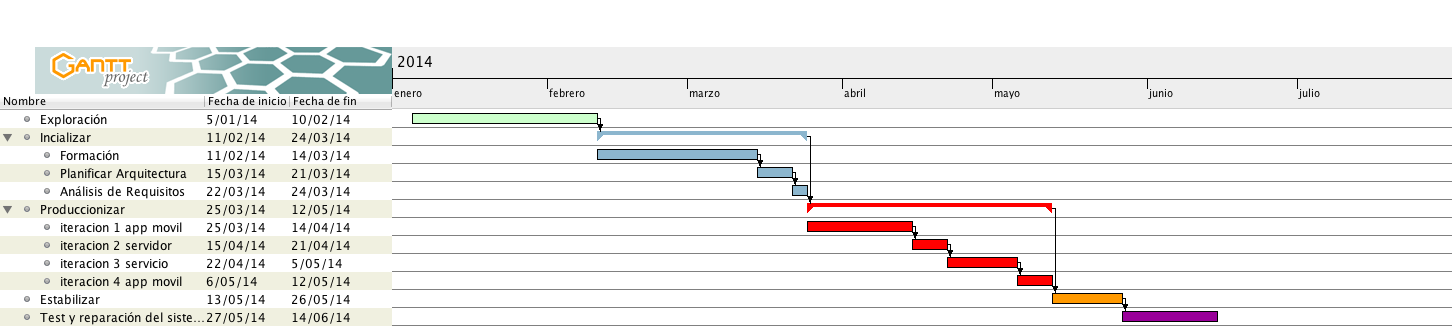
\includegraphics[angle=90,scale=0.45]{diagramagantt.png}
  \caption{Diagrama de Gantt (versión 1.0)}
\end{figure}
\subsection{Organización}
    	Todos los roles definidos para la organización del proyecto se han asignado de acuerdo con la metodología \textit{Mobile-D}\cite{AgileMobileD}.
\paragraph{Grupo de cliente}Inicialmente se procederá a identificar al \textit{cliente} del proyecto. Se plantea como finalidad del proyecto: ofrecer una solución a una problemática existente por parte del Ayuntamiento de Puerto Real en lo referido a la recogida de muebles y otros enseres. Se hace necesario el establecer como cliente al responsables del área de sistemas informáticos y a encargado de la gestión logística de limpieza y operaciones de recogida de muebles. Por lo tanto, se establecen como responsables de la comunicación con la entidad cliente al \textit{Analista de Sistema del Ayuntamiento de Puerto Real} y al \textit{Responsable de operativa del grupo Epresa21}. Como vía de contacto se incluye la dirección de correo electrónico del analista de sistemas quien tiene contacto directo con el responsable de operativa. Se definen para cada uno de los responsables de comunicación una serie de funciones:

\begin{itemize}
    \item \textit{Analista de Sistemas: }se dirigirán a él todo tipo de consultas técnicas referidas a la aplicación, servidor, comunicaciones e interfaz gráfica. Se informará de la evolución técnica del proyecto, y se efectuará entrega del producto una vez se encuentre en una versión funcional.
    \item \textit{Responsable de operativa: }todo lo referido a operativas, funcionamiento interno, datos a manejar deberá ser consultado al responsable de operativa. Así mismo se corroboran todos los aspectos de lógica de negocio.
\end{itemize}


% Roles alumno
\paragraph{Roles asociados al alumno autor del TFG}Debido a que dicho proyecto se ha realizado de manera individual, todos estos roles han sido asumidos por el propio alumno autor del proyecto. Se explica a continuación cada una de las finalidades de dichos roles:

\begin{itemize}
    \item \textbf{Equipo de exploración: }grupo encargado de realizada la fase de exploración del proyecto. En este caso la totalidad de la fase de exploración será realizada por el alumno autor del proyecto. 
    \item\textbf{Equipo de proyecto: }equipo de desarrollo del proyecto. Además de las actividades de desarrollo se incluye actividades de arquitectura, testear y recolectar métricas. Todas las tareas anteriormente enumeradas serán llevadas a cabo únicamente por el alumno autor del proyecto.
    \item \textbf{Grupo directivo: }encargado de realizar la toma decisiones referentes al proyecto. Todas las decisiones finales referidas al proyecto, aunque consultadas con el cliente, serán tomadas por el alumno autor del proyecto.
    \item \textbf{Grupo de soporte: }subroles requeridos a lo largo del proyecto. Se contempla la inclusión externa de colaboración para la elaboración de la interfaz gráfica de la app.
    \item \textbf{Grupo de test del sistema: }las pruebas del sistema serán realizadas por el alumno autor del proyecto.
    \item \textbf{Secretario: }se encargará de crear y mantener un listado de las acciones que se van a realizar, y actualizarlos en función del progreso del proyecto. 
\end{itemize}

% Roles tutora
\paragraph{Roles asociados a la tutora del proyecto}siguiente la metodología se asignan a la tutora del proyecto los siguientes roles:
\begin{itemize}
    \item \textbf{Moderador: }la metodología nos indica que es preferible que sea alguien fuera del equipo de proyecto. Se encargará de agrupar los resultados, comprobar el cumplimiento del calendario y gestionar discusiones. Además debe de ser un punt o de unión entre el estado del proyecto y la organización. 
    \item \textbf{Auditor Externo: }persona quién realizará las auditorías y detectará deficiencias. Decidirá si los resultados son válidos y aceptables. El auditor debe tener conocimiento del proyecto. 
\end{itemize}
\subsection{Costes}
\subsection{Gestión de riesgos}

\chapter{Desarrollo}
\section{Análisis de Requisitos}
\subsection{Catálogo de actores}
	\begin{table}[h]
\centering
\begin{tabular}{|c|l|l}
\cline{1-2}
\textbf{ACT-0001}    & \multicolumn{1}{|c|}{\textbf{Usuario}}                                                                                                                    &  \\ \cline{1-2}
\textbf{Versión}     & 1.0 (20/03/2014)                                                                                                                                            &  \\ \cline{1-2}
\textbf{Fuente}      & Epresa21                                                                                                                                                    &  \\ \cline{1-2}
\textbf{Descripción} & \begin{tabular}[c]{@{}c@{}}Este actor representa a cada uno de los usuarios de la aplicación \\ de recogida de enseres.\end{tabular}                        &  \\ \cline{1-2}
\textbf{Comentario}  & \begin{tabular}[c]{@{}c@{}}previa petición de los mismos al teléfono 956 880 884 o bien \\ solicitud web mediante portal web del ayuntamiento.\end{tabular} &  \\ \cline{1-2}
\end{tabular}
\caption{ACT-0001 Usuario}
\end{table}
	\begin{table}[h]
\centering
\begin{tabular}{|c|l|l}
\cline{1-2}
\textbf{ACT-0002}    & \multicolumn{1}{|c|}{\textbf{Operador}}                                                                                                                                                                                          &  \\ \cline{1-2}
\textbf{Versión}     & 1.0 (20/03/2014)                                                                                                                                                                                                                 &  \\ \cline{1-2}
\textbf{Fuente}      & Epresa21                                                                                                                                                                                                                         &  \\ \cline{1-2}
\textbf{Descripción} & \begin{tabular}[c]{@{}c@{}}Este actor representa al operador que consulta desde la sede de la\\ \\ empresa las peticiones de recogida realizadas y realiza informes\\ mensuales cuando lo solicita el ayuntamiento.\end{tabular} &  \\ \cline{1-2}
\textbf{Comentario}  & \begin{tabular}[c]{@{}c@{}}Dicho usuario pertenece a la localidad en la que se proporciona\\ el servicio.\end{tabular}                                                                                                           &  \\ \cline{1-2}
\end{tabular}
\caption{ACT-0002 Operador}
\end{table}
	
\subsection{Requisitos funcionales}
\subsubsection*{Casos de uso del sistema}
	\begin{figure}[H]
	\centering
 	   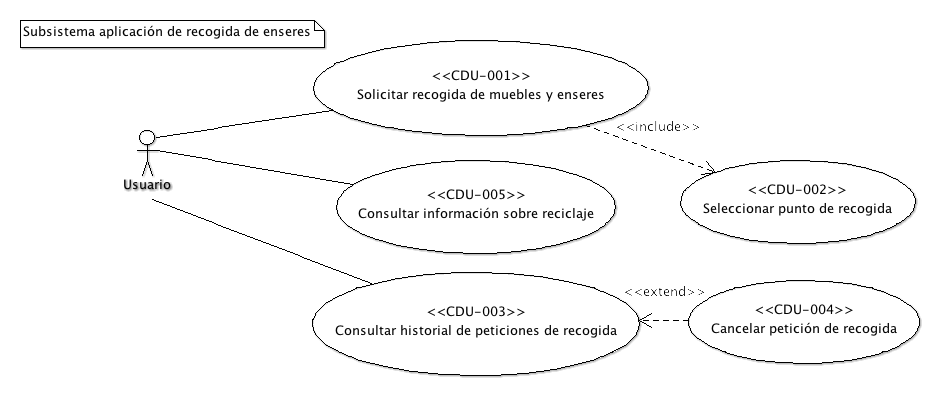
\includegraphics[scale=0.50]{diagramaCU1.png} 
  	  \caption{Diagrama UML del Subsistema aplicación de recogida de muebles y enseres.}
	\end{figure}	
	% CDU-001: Solicitar recogida de muebles y ensere
\begin{longtable}{p{2.5cm}  p{14cm}}
\caption*{\textbf{CDU-001: Solicitar recogida de muebles y enseres}} \\
\hline
\textbf{Versión} & 1.0 (26/03/2014) \\
\textbf{Fuentes} & Apresa21 \\
\textbf{Dependencias} & OBJ-001 CDU-002 \\
% Descripción del caso de uso
\textbf{Descripción} & El sistema deberá comportarse tal como se describe en el siguiente caso de uso cuando \textit{un usuario desee solicitar la recogida de uno o varios muebles y enseres.} \\
\textbf{Frecuencia esperada} & 10 veces al día \\
\textbf{Importancia} & Vital  \\
\textbf{Comentarios} &- \\
\end{longtable}

\textbf{Secuencia Normal} 
\begin{enumerate}
	\item[1.] El actor \textit{Usuario (ACT-0001)} solicita al sistema la recogida de uno o varios muebles y enseres.
	\item[2.] El \textit{Sistema} solicita al \textit{Usuario (ACT-0001)} que indique qué tipo de mueble o enser quiere depositar para su recogida, así como el volumen de dicho objeto.
	% Excepción en el paso 3
	\item[3.] El actor \textit{Usuario (ACT-0001)} indica qué tipo de mueble o enser va a depositar así como las características del mismo (Repetir este paso hasta que se hayan incluido todos los objetos que el actor \textit{Usuario (ACT-0001)} desea depositar para su posterior recogida).
	\item[4.] Seleccionar punto donde se depositarán los muebles y enseres para su posterior recogida. \textbf{Include (Seleccionar punto de recogida)}

	\item[5.] El \textit{Sistema} comprueba la primera fecha disponible para registrar la cita para recogida de los muebles y enseres.
	% Excepción en el paso 6
	\item[6.] El \textit{Sistema} comprueba si se han solicitado más del número máximo de objetos al día que se pueden recoger. Se han solicitado menos del número máximo de objetos por usuario al día que se pueden solicitar para que sean recogidas. Adicionalmente se comprueba si es posible dar respuesta a la recogida de objetos dentro del cupo de recogida 	diaria para dicha fecha. Se comprueba que es posible recoger todos los enseres en el mismo día.
	\item[7.] El \textit{Sistema} muestra al usuario las instrucciones que debe seguir para depositar los muebles y enseres. Una vez mostradas muestra la fecha y localización de la recogida y solicita confirmación.
	\item[8.] El actor \textit{Usuario (ACT-0001)} visualiza todas las instrucciones y confirma la recogida de muebles y enseres.
	\item[9.] El \textit{Sistema} registra en el sistema la fecha de recogida y el número de enseres, así como la ubicación.
	\item[10.] El \textit{Sistema} muestra al usuario una confirmación a la solicitud de recogida de muebles y enseres con la fecha y lugar donde serán recogidos.
\end{enumerate} 

\textbf{Postcondición: } 
 Se registra la solicitud de recogida de muebles y enseres con la ubicación y fecha(s).\\

\textbf{Excepciones} 
\begin{enumerate}
\item[*a.] El actor \textit{Usuario (ACT-0001)} cancela el proceso de solicitud de recogida de muebles y enseres.
	\begin{enumerate}
		\item[1.] El Sistema cancela el registro de la solicitud de recogida de muebles y enseres.
	\end{enumerate}
\item[3a.] El actor \textit{Usuario (ACT-0001)} desea solicitar la recogida de más de un mueble o enser.
	\begin{enumerate}
		 \item[1.] El actor \textit{Usuario (ACT-0001)} vuelve a indicar que tipo de mueble o enser va a depositar así como las características del mismo.
		 \item[2.] EL \textit{Sistema} incluye el objeto en el listado de muebles y enseres que el usuario desea que sean recogidos para reciclar.
		 \item[3.] EL \textit{Sistema} comprueba si se ha superado el máximo número de muebles y enseres que se pueden recoger por usuario al día. En caso afirmativo muestra un mensaje al usuario informando que el máximo número de objetos que se recogen por día es ese y que la recogida se hará en varias jornadas.
	\end{enumerate}
\item[3b.] El actor \textit{Usuario (ACT-0001)} desea solicitar la recogida de un mueble o enser que no esta en el listado de productos recogidas y cuyas características no se pueden indicar.
	\begin{enumerate}
		\item[1.] El \textit{Sistema} informa al usuario que debe ponerse en contacto con el número de teléfono de la empresa municipal (Se finaliza el caso de uso).
	\end{enumerate}	
\item[6a.] El \textit{Sistema} comprueba que no es posible dar servicio en un solo día a la petición del usuario al sobrepasar el número de objetos que pueden recogerse en un día o en el primer día disponible.
	\begin{enumerate}
		\item[1.] El Sistema organiza la recogida en varios días teniendo el cuenta el máximo número de objetos que se recogen por día y usuario y el número de objetos que se van a recoger en la primera fecha disponible. Vuelve al paso 11.
	\end{enumerate}
\item[9a.] El \textit{Sistema} no puede registrar  en el sistema la fecha de recogida y el número de enseres, así como la ubicación.
	\begin{enumerate}
		\item[1.] El \textit{Sistema} informa de que no ha sido posible resolver la solicitud del usuario y que debe ponerse en contacto con el Teléfono de contacto de la empresa de recogida de muebles y enseres.
	\end{enumerate}
\end{enumerate}

	% CDU-002: Seleccionar punto de recogida
\begin{longtable}{p{2.5cm}  p{14cm}}
\caption*{\textbf{CDU-002: Seleccionar punto de recogida}} \\
\hline
\textbf{Versión} & 1.0 (26/03/2014) \\
\textbf{Fuentes} & Apresa21 \\
\textbf{Dependencias} & OBJ-001 CDU-001 \\
% Descripción del caso de uso
\textbf{Descripción} & El sistema deberá comportarse tal como se describe en el siguiente caso de uso cuando \textit{haya que seleccionar una ubicación donde el usuario depositará sus muebles y enseres para que posteriormente sean recogidos por el camión de la empresa de reciclaje.} \\
\textbf{Frecuencia esperada} & 10 veces al día \\
\textbf{Precondición} & El terminal móvil del usuario dispone de tecnología GPS funcional y con cobertura. \\
\textbf{Importancia} & Vital  \\
\textbf{Comentarios} & Se establece como distancia máxima del domicilio del cliente 300 metros del punto de depósito de los mueble y enseres. Para distancias mayores se remite al usuario a contactar vía telefónica con la empresa de recogida de muebles y enseres. \\
\end{longtable}

\textbf{Secuencia Normal} 
\begin{enumerate}
	\item[1.] El \textit{Sistema} solicita al usuario si desea introducir su dirección manualmente o bien ser geolocalizado mediante el sistema de localización GPS del propio terminal móvil.
	% Excepción en el paso 2
	\item[2.] El actor \textit{Usuario (ACT-0001)} introduce indica que desea introducir manualmente el punto de recogida, introduce su calle y número.
	% Excepción en el paso 3
	\item[3.] El \textit{Sistema} comprueba si la localización corresponde al término municipal donde se oferta el servicio de recogida de muebles y enseres.
	\item[4.] El \textit{Sistema} comprueba si el punto de recogida se encuentra a menos de 300 metros del domicilio del usuario y muestra al usuario el punto de recogida más cercano a su domicilio. 
	\item[5.] El \textit{Sistema} comprueba si la localización corresponde a una zona rural o una zona urbana del término municipal. Es una zona urbana. 
\end{enumerate}

\textbf{Postcondición: } 
 Se obtiene el punto donde de recogida donde el usuario depositará los muebles y enseres.\\

\textbf{Excepciones} 
\begin{enumerate}
	\item[2a.] El actor \textit{Usuario (ACT-0001)} desea emplear la localización por medio del servicio GPS de su terminal móvil.
	\begin{enumerate}
		\item[1.] El Sistema solicita al terminal móvil la ubicación GPS en la cual se encuentra en ese mismo instante.
		\item[2.] El Sistema obtiene las coordenadas del domicilio del usuario por medio del servicio de localización GPS. Vuelve al paso 3.
	\end{enumerate}
	\item[3a.] El \textit{Sistema} comprueba que la localización está fuera del término municipal donde se oferta el servicio de recogida de muebles y enseres.
	\begin{enumerate}
		\item[1.] El \textit{Sistema} informa al usuario que actualmente el servicio solo se oferte en dicho término municipal y que no es posible prestarle el servicio. Se finaliza el caso de uso.
	\end{enumerate}
	\item[4a.] El \textit{Sistema} comprueba que todos los puntos de recogida están a más de 300 metros del domicilio del usuario que solicita el servicio.
	\begin{enumerate}
		\item[1.] El \textit{Sistema} informa al usuario que debe ponerse en contacto con el número de teléfono de la empresa municipal. Se finaliza el caso de uso.
	\end{enumerate} 	
\end{enumerate} 

	% CDU-003: Consultar Historial de Peticiones de Recogida
\begin{longtable}{p{2.5cm}  p{14cm}}
\caption*{\textbf{CDU-003: Consultar Historial de Peticiones de Recogida}} \\
\hline
\textbf{Versión} & 1.0 (26/03/2014) \\
\textbf{Fuentes} & Apresa21 \\
\textbf{Dependencias} & OBJ-001 \\
% Descripción del caso de uso
\textbf{Descripción} & El sistema deberá comportarse tal como se describe en el siguiente caso de uso cuando \textit{un usuario desee consultar las peticiones de recogida de uno o varios muebles y enseres que ha solicitado anteriormente.} \\
\textbf{Frecuencia esperada} & 1 veces a la semana  \\
\textbf{Precondición} & El actor \textit{Usuario (ACT-0001)} ha realizado anteriormente una o varios solicitudes de recogida de mueble y enseres. \\
\textbf{Importancia} & Baja  \\
\textbf{Comentarios} &- \\
\end{longtable}

\textbf{Puntos de extensión:} 
borrar en 3a. \\

\textbf{Secuencia Normal} 
\begin{enumerate}
	\item[1.] El actor \textit{Usuario (ACT-0001)} desea consultar las solicitudes que ha realizado de recogida de muebles y enseres.
	\item[2.] El sistema consulta las peticiones de recogida de muebles y enseres que tiene pendiente y las que ha realizado anteriormente y las muestra por pantalla.
	\item[3] El actor \textit{Usuario (ACT-0001)} selecciona una petición para visualizar mas detalles.
\end{enumerate}

\textbf{Postcondición: } 
 Se muestran por pantalla las peticiones de recogida de muebles y enseres que ha realizado el usuario.\\

\textbf{Excepciones} 
\begin{enumerate}
	\item[3a.] El actor \textit{Usuario (ACT-0001)} desea cancelar una petición que ha solicitado y que aún está pendiente de resolución.
\end{enumerate} 	
	% CDU-004: Cancelar petición de recogida
\begin{longtable}{p{2.5cm}  p{14cm}}
\caption*{\textbf{CDU-004: Cancelar petición de recogida}} \\
\hline
\textbf{Versión} & 1.0 (26/03/2014) \\
\textbf{Fuentes} & Apresa21 \\
\textbf{Dependencias} & OBJ-001 CDU-003 \\
% Descripción del caso de uso
\textbf{Descripción} & El sistema deberá comportarse tal como se describe en el siguiente caso de uso cuando \textit{un Usuario desee cancelar una solicitud de recogida de muebles y enseres que tiene pendiente para los próximos días.} \\
\textbf{Frecuencia esperada} & 1 vez al mes  \\
\textbf{Precondición} & El actor \textit{Usuario (ACT-0001)} ha realizado anteriormente una o varios solicitudes de recogida de mueble y enseres. Dicha solicitud se realizará en una fecha posterior a la fecha del Sistema. \\
\textbf{Importancia} & Baja  \\
\textbf{Comentarios} & Sólo se cancelarán las peticiones de recogidas de enseres pendiente, con fechas posteriores a la fecha actual del Sistema. \\
\end{longtable}

\textbf{Secuencia Normal} 
\begin{enumerate}
	\item[1.] El actor \textit{Usuario (ACT-0001)} desea cancelar una petición, anteriormente seleccionada y pendiente de realizar, para que le recojan muebles y enseres.
	\item[2.] El \textit{Sistema} muestra un mensaje al usuario confirmando la eliminación de la petición de recogida de muebles y enseres.
	\item[3.] El actor \textit{Usuario (ACT-0001)} confirma su deseo de eliminar la petición.
	\item[4.] El \textit{Sistema} elimina la petición de recogida de muebles y enseres de los registros de solicitudes y actualiza el histórico de solicitudes de recogida de muebles y enseres.
\end{enumerate}
	% CDU-005: Consultar información sobre reciclaje
\begin{longtable}{p{2.5cm}  p{14cm}}
\caption*{\textbf{CDU-005: Consultar información sobre reciclaje}} \\
\hline
\textbf{Versión} & 1.0 (27/03/2014) \\
\textbf{Fuentes} & Apresa21 \\
\textbf{Dependencias} & OBJ-002 \\
% Descripción del caso de uso
\textbf{Descripción} & El sistema deberá comportarse tal como se describe en el siguiente caso de uso cuando \textit{un usuario solicita información sobre información útil sobre el reciclaje, todas sus aplicaciones, ventajas y beneficios para el medioambiente.} \\
\textbf{Frecuencia esperada} & 30 veces a la semana  \\
\textbf{Precondición} & - \\
\textbf{Importancia} & Baja  \\
\textbf{Comentarios} &- \\
\end{longtable}

\textbf{Secuencia Normal} 
\begin{enumerate}
	\item[1.] El actor \textit{Usuario (ACT-0001)} consulta información sobre el reciclaje y todas sus aplicaciones ventajas y beneficios para el medioambiente.
	\item[2.] El \textit{Sistema} muestra la información agrupada en función del tipo de residuo.
	\item[3.] El actor \textit{Usuario (ACT-0001)} elige un tipo de residuo.
	\item[4.] El \textit{Sistema} muestra la información disponible sobre dicho residuo.
\end{enumerate}	
	
	\begin{figure}[H]
	\centering
 	   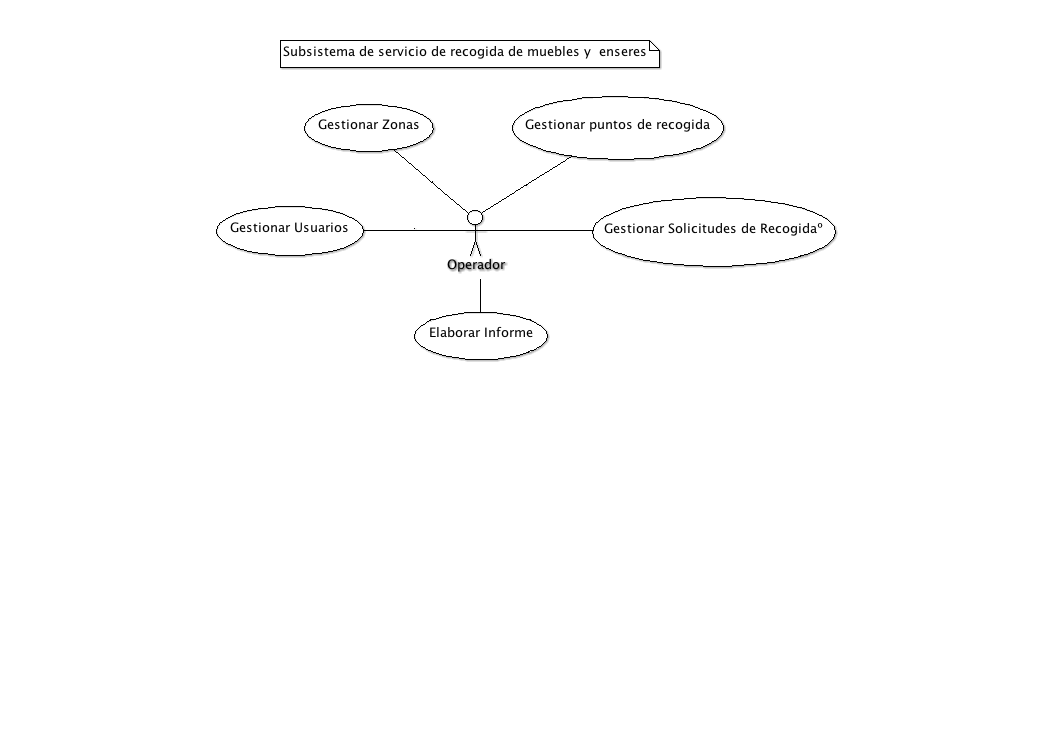
\includegraphics[scale=0.50]{diagramaCU2.png} 
  	  \caption{Diagrama UML del Subsistema de servicio de recogida de muebles y enseres.}
	\end{figure}	

\subsection{Requisitos de información}
	% Información sobre enseres
\begin{center}
\begin{longtable}{|p{80pt}|p{9cm}|}
\hline
\textbf{IRQ-001} & Información sobre Enseres \\ \hline
\textbf{Dependencias} & OBJ-001 \\ \hline
\textbf{Descripción} & El sistema deberá almacenar la información correspondiente a los Tipos de Enseres que se vayan a recoger de cara a planificar las rutas del camión. En concreto: \\ \hline
\textbf{Datos \mbox{específicos}} & 
\begin{itemize}
    \item Nombre del enser ( \textit{Identificador del objeto que se debe recoger} )
    \item Volumen ( \textit{Aproximado en metros cúbicos} )
    \item Altura ( \textit{Aproximado en metros cúbicos} )
    \item Anchura ( \textit{Aproximado en metros cúbicos} )
    \item Peso ( \textit{Aproximado en kilogramos} )
\end{itemize}\\ \hline
\caption{IRQ-001  Información sobre Enseres}
\end{longtable}
\end{center}
	% Unicidad de Enseres
\begin{center}
\begin{longtable}{|p{80pt}|p{9cm}|}
\hline
\textbf{CRQ-001} & Unicidad de Enseres \\ \hline
\textbf{Dependencias} & OBJ-001 \\ \hline
\textbf{Descripción} & La información almacenada por el sistema deberá satisfacer la siguiente restricción: todas los enseres tendrán un Nombre de enser único. \\ \hline
\caption{CRQ-001 Unicidad de Enseres}
\end{longtable}
\end{center}

	% Información sobre usuarios
\begin{center}
\begin{longtable}{|p{80pt}|p{9cm}|}
\hline
\textbf{IRQ-002} & Información sobre Usuarios \\ \hline
\textbf{Dependencias} & OBJ-001 y OBJ-003 \\ \hline
\textbf{Descripción} & El sistema deberá almacenar la información correspondiente Usuarios que solicitan la recogida de enseres. En concreto: \\ \hline
\textbf{Datos \mbox{específicos}} & 
\begin{itemize}
    \item Nombre del Usuario ( \textit{Identificador del usuario que solicita la recogida de muebles o enseres} )
    \item Apellidos del Usuario ( \textit{Sus apellidos, este campo es opcional} )
    \item Teléfono de contacto ( \textit{El número de teléfono del móvil desde el que tiene instalada la aplicación} )
    \item Identificador ( \textit{Un número que identifique al usuario de forma unívoca} )
\end{itemize}\\ \hline
\caption{IRQ-002  Información sobre Usuarios}
\end{longtable}
\end{center}
	% Unicidad de Usuarios
\begin{center}
\begin{longtable}{|p{80pt}|p{9cm}|}
\hline
\textbf{CRQ-002} & Unicidad de Usuarios \\ \hline
\textbf{Dependencias} & OBJ-001 y OBJ-003 \\ \hline
\textbf{Descripción} & La información almacenada por el sistema deberá satisfacer la siguiente restricción: todas los Usuarios tendrán un Identificador de Usuario único. \\ \hline
\caption{CRQ-002 Unicidad de Usuarios}
\end{longtable}
\end{center}
	
	% Información sobre recogidas de enseres
\begin{center}
\begin{longtable}{|p{80pt}|p{9cm}|}
\hline
\textbf{IRQ-003} & Información sobre las  Solicitudes de recogidas de muebles y enseres \\ \hline
\textbf{Dependencias} & OBJ-001 y OBJ-003 \\ \hline
\textbf{Descripción} & El sistema deberá almacenar la información correspondiente las solicitudes de recogidas de muebles de enseres. En concreto: \\ \hline
\textbf{Datos \mbox{específicos}} & 
\begin{itemize}
    \item Identificador de solicitud ( \textit{Identificador de solicitud de recogida de muebles o enseres} )
    \item Usuario solicitante ( \textit{Identificador de usuario que solicita la recogida de muebles o enseres} )
    \item Fecha ( \textit{Fecha en la que se estipula la recogida de los muebles y enseres} )
    \item Punto de recogida ( \textit{Ubicación en la que se depositarán los muebles y enseres} )
    \item Tipo de muebles y enseres depositados ( \textit{Tipo de muebles y enseres que se depositarán en el punto de recogida} )
\end{itemize}\\ \hline
\caption{IRQ-003 Información sobre las solicitudes de recogidas de muebles y enseres}
\end{longtable}
\end{center}
	% Unicidad de solicitudes de recogida de muebles y enseres
\begin{center}
\begin{longtable}{|p{80pt}|p{9cm}|}
\hline
\textbf{CRQ-003} & Unicidad de solicitudes de recogida de muebles y enseres \\ \hline
\textbf{Dependencias} & OBJ-001 y OBJ-003 \\ \hline
\textbf{Descripción} & La información almacenada por el sistema deberá satisfacer la siguiente restricción: todas los solicitudes de recogidas de muebles y enseres tendrán un Identificador de solicitud único. \\ \hline
\caption{CRQ-003 Unicidad de solicitudes de recogida de muebles y enseres}
\end{longtable}
\end{center}
	
	% Información sobre los puntos de recogida
\begin{center}
\begin{longtable}{|p{80pt}|p{9cm}|}
\hline
\textbf{IRQ-004} & Información sobre los puntos de recogida \\ \hline
\textbf{Dependencias} & OBJ-001 \\ \hline
\textbf{Descripción} & El sistema deberá almacenar la información correspondiente los puntos de recogida de muebles y enseres. En concreto: \\ \hline
\textbf{Datos \mbox{específicos}} & 
\begin{itemize}
    \item Identificador de solicitud ( \textit{Identificador de solicitud de recogida de muebles o enseres} )
    \item Zona ( \textit{Si es zona rural o zona urbana} )
    \item Posición ( \textit{localización gps del punto de recogida} )
\end{itemize}\\ \hline
\caption{IRQ-004Información sobre los puntos de recogida}
\end{longtable}
\end{center}
	
	\newpage
	\subsubsection*{Diagrama conceptual de clases UML}
	\begin{figure}[H]
	\centering
 	   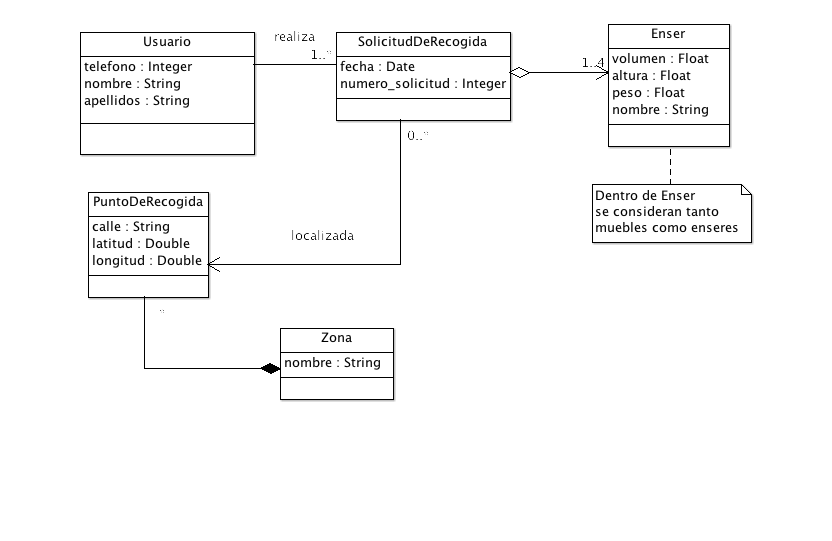
\includegraphics[scale=0.70,angle =90]{diaConceptualUML.png} 
  	  \caption{Diagrama conceptual de clases UML.}
	\end{figure}
	
	\newpage
	\subsubsection*{Tipos}
	% Tipo Usuario
	% Tipo que representa USUARIOS

\begin{longtable}{p{2.5cm}  p{14cm}}
\caption*{\textbf{TYP-001: Usuario}} \\
\hline
\textbf{Versión} & 1.0 (31/03/2014) \\
\textbf{Fuentes} & Apresa21 \\
% Descripción del Tipo
\textbf{Descripción} & Este tipo de objetos representa  \textit{los usuarios que solicitan recogida de muebles o enseres} \\
\textbf{Supertipo} & - \\
\textbf{Subtipo} & -  \\
\textbf{Comentarios} &- \\
\end{longtable}

\begin{longtable}{p{3cm}  p{12cm}}
\hline
\textbf{Atributo variable} & Usuario::teléfono \\
% Descripción del Atributo
\textbf{Descripción} & Este atributo representa  \textit{el número de teléfono del usuario} \\
\textbf{Tipo} & \textit{String} \\
\textbf{Comentarios} & Este campo se empleará para identificar al usuario. El teléfono es un teléfono de móvil. En caso de que haya alguna incidencia se contactará a este número. \\
\end{longtable}

\begin{longtable}{p{3cm}  p{12cm}}
\hline
\textbf{Atributo variable} & Usuario::Nombre \\
% Descripción del Atributo
\textbf{Descripción} & Este atributo representa  \textit{el nombre del solicitante del servicio de recogida y del titular del teléfono móvil.} \\
\textbf{Tipo} & \textit{String} \\
\textbf{Comentarios} &- \\
\end{longtable}

\begin{longtable}{p{3cm}  p{12cm}}
\hline
\textbf{Atributo variable} & Usuario::Apellidos \\
% Descripción 
\textbf{Descripción} & Este atributo representa  \textit{los apellidos del solicitante del servicio de recogida y titular del teléfono móvil.} \\
\textbf{Tipo} & \textit{String} \\
\textbf{Comentarios} & Este campo es opcional \\
\end{longtable}

\begin{longtable}{p{3cm}  p{12cm}}
\hline
\textbf{Expresión de invariante} & Usuario de teléfono \\
% Descripción 
\textbf{Descripción} & No puede haber Usuarios con el mismo teléfono en el Sistema. \\
\textbf{Comentarios} & - \\
\end{longtable}

	% Tipo SolicitudRecogida	
	% Tipo que representa SOLICITUDES DE RECOGIDA

\begin{longtable}{p{2.5cm}  p{14cm}}
\caption*{\textbf{TYP-002: SolicitudRecogida}} \\
\hline
\textbf{Versión} & 1.0 (31/03/2014) \\
\textbf{Fuentes} & Apresa21 \\
\textbf{Descripción} & Este tipo de objetos representa  \textit{la solicides de recogidas de muebles y enseres realizadas por los usuarios} \\
\textbf{Supertipo} & - \\
\textbf{Subtipo} & -  \\
\textbf{Comentarios} &- \\
\end{longtable}

% Atributos
\begin{longtable}{p{3cm}  p{12cm}}
\hline
\textbf{Atributo variable} & SolicitudRecogida::fecha \\
\textbf{Descripción} & Este atributo representa  \textit{la fecha en la cual se establece la solicitud de recogida.} \\
\textbf{Tipo} & \textit{String} \\
\textbf{Comentarios} & - \\
\end{longtable}

\begin{longtable}{p{3cm}  p{12cm}}
\hline
\textbf{Atributo variable} & SolicitudRecogida::numeroSolicitud \\
\textbf{Descripción} & Este atributo representa  \textit{el número de solicitud.} \\
\textbf{Tipo} & \textit{Natural} \\
\textbf{Comentarios} & Este atributo es identifica y sirve para contabilizar el número de solicitudes realizadas. \\
\end{longtable}

% Invariantes
\begin{longtable}{p{3cm}  p{12cm}}
\hline
\textbf{Expresión de invariante} & SolicitudRecogida::UnicidadnumeroSolicitud \\
\textbf{Descripción} &  \textit{No puede haber dos solicitudes de recogida con el mismo número} \\
\textbf{Comentarios} & -\\
\end{longtable}
	
	% Tipo PuntosDeRecogida	
	% Tipo que representa PUNTOS DE RECOGIDA

\begin{longtable}{p{2.5cm}  p{14cm}}
\caption*{\textbf{TYP-003: puntoRecogida}} \\
\hline
\textbf{Versión} & 1.0 (01/04/2014) \\
\textbf{Fuentes} & Apresa21 \\
\textbf{Descripción} & Este tipo de objetos representa  \textit{los puntos de recogida donde se depositarán los muebles y enseres para su posterior recogida.} \\
\textbf{Supertipo} & - \\
\textbf{Subtipo} & -  \\
\textbf{Comentarios} &- \\
\end{longtable}

% Atributos
\begin{longtable}{p{3cm}  p{12cm}}
\hline
\textbf{Atributo variable} & puntoRecogida::calle \\
\textbf{Descripción} & Este atributo representa  \textit{el nombre de la calle donde esta ubicado el punto de recogida.} \\
\textbf{Tipo} & \textit{String} \\
\textbf{Comentarios} & - \\
\end{longtable}

\begin{longtable}{p{3cm}  p{12cm}}
\hline
\textbf{Atributo variable} & puntoRecogida::latitud \\
\textbf{Descripción} & Este atributo representa  \textit{la latitud de la coordenada en la que se encuentra el punto de recogida} \\
\textbf{Tipo} & \textit{Double} \\
\textbf{Comentarios} & - \\
\end{longtable}

\begin{longtable}{p{3cm}  p{12cm}}
\hline
\textbf{Atributo variable} & puntoRecogida::longitud \\
\textbf{Descripción} & Este atributo representa  \textit{la longitud de la coordenada en la que se encuentra el punto de recogida} \\
\textbf{Tipo} & \textit{Double} \\
\textbf{Comentarios} & - \\
\end{longtable}

% Invariantes
\begin{longtable}{p{3cm}  p{12cm}}
\hline
\textbf{Expresión de invariante} & SolicitudRecogida::UnicidadLatitudLongitud \\
\textbf{Descripción} &  \textit{No existirán dos puntos de recogida ubicados en la misma coordenada, es decir que posean la misma latitud y longitud. } \\
\textbf{Comentarios} & -\\
\end{longtable}		
	% Tipo Zonas	
	% Tipo que representa ZONAS

\begin{longtable}{p{2.5cm}  p{14cm}}
\caption*{\textbf{TYP-004: zonas}} \\
\hline
\textbf{Versión} & 1.0 (01/04/2014) \\
\textbf{Fuentes} & Apresa21 \\
\textbf{Descripción} & Este tipo de objetos representa  \textit{las distintas zonas del municipio en el que se ofrece el servicio de recogida de muebles y enseres.} \\
\textbf{Supertipo} & - \\
\textbf{Subtipo} & -  \\
\textbf{Comentarios} &- \\
\end{longtable}

% Atributos
\begin{longtable}{p{3cm}  p{12cm}}
\hline
\textbf{Atributo variable} & zonas::nombre \\
\textbf{Descripción} & Este atributo representa  \textit{el nombre de la zona del municipio.} \\
\textbf{Tipo} & \textit{String} \\
\textbf{Comentarios} & - \\
\end{longtable}

% Invariantes
\begin{longtable}{p{3cm}  p{12cm}}
\hline
\textbf{Expresión de invariante} & zonas::UnicidadDelNombre \\
\textbf{Descripción} &  \textit{No existirán dos zonas con el mismo nombre}.  \\
\textbf{Comentarios} & -\\
\end{longtable}
	% Tipo Enseres	
	% Tipo que representa ENSERES

\begin{longtable}{p{2.5cm}  p{14cm}}
\caption*{\textbf{TYP-005: Enser}} \\
\hline
\textbf{Versión} & 1.0 (01/04/2014) \\
\textbf{Fuentes} & Apresa21 \\
\textbf{Descripción} & Este tipo de objetos representa  \textit{los distintos enseres que los Usuarios entregan para que sean recogidos por la empresa de reciclaje.} \\
\textbf{Supertipo} & - \\
\textbf{Subtipo} & -  \\
\textbf{Comentarios} &- \\
\end{longtable}

% Atributos
\begin{longtable}{p{3cm}  p{12cm}}
\hline
\textbf{Atributo variable} & Enser::nombre \\
\textbf{Descripción} & Este atributo representa  \textit{el nombre del enser.} \\
\textbf{Tipo} & \textit{String} \\
\textbf{Comentarios} & - \\
\end{longtable}

% Atributos
\begin{longtable}{p{3cm}  p{12cm}}
\hline
\textbf{Atributo variable} & Enser::altura \\
\textbf{Descripción} & Este atributo representa  \textit{la altura aproximada del enser en metros} \\
\textbf{Tipo} & \textit{Float} \\
\textbf{Comentarios} & - \\
\end{longtable}

% Atributos
\begin{longtable}{p{3cm}  p{12cm}}
\hline
\textbf{Atributo variable} & Enser::peso \\
\textbf{Descripción} & Este atributo representa  \textit{el peso aproximada del enser en kilogramos} \\
\textbf{Tipo} & \textit{Float} \\
\textbf{Comentarios} & - \\
\end{longtable}

% Atributos
\begin{longtable}{p{3cm}  p{12cm}}
\hline
\textbf{Atributo variable} & Enser::volumen \\
\textbf{Descripción} & Este atributo representa  \textit{el volumen aproximado en metros cúbicos} \\
\textbf{Tipo} & \textit{Float} \\
\textbf{Comentarios}
\end{longtable}

% Invariantes
\begin{longtable}{p{3cm}  p{12cm}}
\hline
\textbf{Expresión de invariante} & Enser::UnicidadDelNombre \\
\textbf{Descripción} &  \textit{No existirán dos enseres con el mismo nombre}.  \\
\textbf{Comentarios} & -\\
\end{longtable}	
				
\subsection{Requisitos no funcionales}
% Descripción de otros requisitos (relacionados con la calidad del software) portabilidad, seguridad, auditoría, monitorización, fiabilidad,
% comunicaciones con sistemas externos, extensibilidad, rendimiento, escalabilidad, estándares de obligado cumplimiento, accesibilidad, usabilidad, aspectos de la interfaz de usuario, 
% utilización de un determinado entorno tecnológico, etc.
\subsubsection*{Seguridad}
El servidor donde se almacenarán y procesarán las solicitudes de los usuarios se encuentra ubicado en la Intranet del ayuntamiento. Por seguridad no se debe permitir el acceso directo de la app móvil al servidor, por lo que se hace imprescindible que un servicio se encargue de intermediar entre el servidor y la aplicación del usuario, así como gestionar las diversas peticiones. En todo momento es de vital importancia controlar el aspecto de seguridad en las comunicaciones y conexiones que se establezcan. 

\subsubsection*{Interfaz}
Para poder maximizar el número de descargas de la aplicación y captar una mayor atención se debe cuidar el aspecto estético. La aplicación que se ofrecerá a la ciudadanía no solo debe ser visualmente atractiva sino identificarse con la empresa y la actividad que realiza. Así mismo, la información debe presentarse de una forma resumida y siempre que sea posible acompañada de un apoyo visual por medio de imágenes o iconografía.

\subsubsection{Usabilidad}
Se pretende hacer más cómoda  y fácil de realizar una gestión rutinaria como es la notificación de recogida de enseres. Es por ello importante que la aplicación sea sencilla de utilizar, y no presente ningún reto ni dificultad en su maneja. Se espere llegar a usuarios de toda edad y nivel formativo. 

\subsection{Reglas de negocio}
	% Se recogerán 25 muebles como máximo.
\textbf{Número máximo de muebles y enseres que serán recogimos por dia.} \\
Dada la capacidad del camión se establece que como máximo se puede dar servicio a la recogida de 25 enseres y muebles al día. Si la demanda superase dicha cantidad de peticiones se debería establecer la citación para la recogida en días posteriores. \\

% Número máximo de enseres diarios.
\textbf{Número máximo de muebles y enseres que serán recogimos por usuario/dia.} \\
El servicio de recogida de muebles y enseres para los habitantes de la localidad de Puerto Real, es un servicio proporcionados por una empresa municipal y de carácter gratuito disponible para toda la ciudadanía del término municipal. Es por ello que para que un solo solicitante no acapare todo el servicio de recogido diario se estipula que un usuario no puede realizar la entrega de más de tres muebles y enseres en un mismo día. En el caso de que un usuario desee que se le recojan más de 4 muebles o enseres se le deberá de concertar las citas en varios días, tantos como requiera la cantidad de muebles y enseres a entregar. Es importante recalcar al usuario que el motivo de dicha limitación es el carácter gratuito de dicho servicio prestado por la empresa municipal. \\

% Mensajes de advertencia.
\textbf{Depositar los muebles enseres en un horario posterior a la medianoche para prever actos vandálicos.} \\
Debido a diversos actos vandálicos que han acontecido en años anteriores (Incendio de colchones o muebles de madera, destrozo de electrodomésticos, etc) se debe advertir al usuario que solicite la recogida de muebles y enseres de que el deposito de dichos objetos debe de realizarse a horas posteriores a la medianoche previa al día en el cual se ha concertado la recogida de los enseres. para prever que acontezcan dichos sucesos, de igual manera se le debe de informar que cualquier destrozo provocado por la quema de dichos objetos no será responsabilidad del ayuntamiento ni del servicio de recogida sino del depositante de los objetos. Mediante estas medidas se trata de prever acciones legales y  que los objetos estén depositados en la calle el menos tiempo posible ya que el camión de recogida de muebles y enseres no saldrá a realizar las recogidas hasta las 7 de la madrugada del día siguiente de ser depositados. \\

% Áreas de ciudad y áreas rurales.
\textbf{Áreas de ciudad y áreas rurales.} \\
Se establecen dos tipos de rutas una ruta diaria para la recogida de muebles y enseres en zonas urbanas, considerandos estas zonas del termino municipal dentro del núcleo urbano. Y por otra parte zonas rurales entra las que se incluyen zonas agrarias, campos y viviendas alejadas del núcleo urbano. Estas viviendas tienen capacidad para almacenar muebles y enseres durante mas tiempo y tienen una muy menor población además de precisas menos demanda del servicio de recogida de muebles y enseres. Por lo tanto, se estipula un único día a la semana para prestarle el servicio de recogida de muebles y enseres, siendo la cantidad estipulada por la capacidad del camión, es decir 25 muebles y enseres por día. \\	

\subsection{Estudio de alternativas tecnológicas}
% En esta sección, se debe ofrecer un estudio del arte de las diferentes alternativas tecnológicas que permitan satisfacer los requerimientos del sistema, para luego seleccionar la herramienta o conjunto de herramientas que utilizaremos como base para el software a desarrollar.

\subsection{Análisis GAP}
% Una vez seleccionado el software de base, debemos identificar y medir las diferencias entre lo que proporciona este software y los requisitos definidos
% para el proyecto. El resultado de este análisis permitirá identificar cuáles de éstos requisitos ya están solventados total o parcialmente por el sistema base y cuales tendremos que diseñar e implementar.

\section{Diseño del Sistema}	
\subsection{Diseño de la arquitectura}


\subsubsection{Arquitectura física}
% En este apartado, describimos los principales componentes hardware que forman la arquitectura física de nuestro sistema, recogiendo por un lado los componentes de servidor y los componentes de sistemas externos con los que colabora nuestro sistema y por otro, los componentes hardware de cliente.

\subsubsection{Arquitectura lógica}
% La arquitectura lógica del sistema está formada por los elementos software (servicios, aplicaciones, librerías, frameworks, etc.) que componen el
% software base, más el software desarrollado para cumplir los requisitos de la aplicación. También, se recogen los componentes de sistemas externos con los que interactúa nuestro sistema, así como los componentes software del lado cliente.


\subsubsection{Arquitectura de diseño}
% La arquitectura de diseño especifica la forma en que los artefactos software de más bajo nivel, interactúan entre sí para lograr el
% comportamiento deseado en el sistema. Utilizaremos el patrón arquitectónico Layers (Capas), con el cual estructuramos el sistema en un número apropiado de capas, de forma que todos los componentes de una misma capa trabajan en el mismo nivel de abstracción y los servicios proporcionados por la capa superior utilizan internamente los servicios proporcionados por la capa inmediatamente inferior.
%\textbf*{Capa de presentación} \\
%\textbf*{Capa de negocio} \\
%\textbf*{Capa de integración} \\
%\textbf*{Servicios trasversales} \\

\newpage
\subsection{Diseño de interfaz de usuario}
% En esta sección se especifican las interfaces entre el sistema y el usuario, detallando el aspecto y el comportamiento de las diferentes pantallas e informes, de acuerdo con el entorno tecnológico definido. Con respecto a las pantallas e informes, es preciso realizar un prototipo o mockup gráfico. Junto a estos bocetos hay que definir qué ocurre en los distintos componentes visuales de la interfaz cuando aparecen y qué acciones se disparan cuando el usuario trabaja con ellas.
% Además, es preciso elaborar un diagrama de navegación, reflejando la secuencia de pantallas a las que tienen acceso los diferentes roles de usuario y la conexión entre éstas.

La interfaz de usuario parte de un menú principal del que parten las diversas opciones. Siempre que el usuario cancele una operación o finalice una petición volverá a este menú principal.
La petición de una solicitud de recogida es una secuencia de pasos en los cuáles el usuario indica qué enseres desea que se le recojan, seguidamente facilita el punto de recogida más cercano de donde tiene los enseres (que habitualmente es su domicilio), acto seguido se informa de las condiciones de uso del servicio y de que sus datos de nombre y teléfono quedarán registrado en el sistema acorde con la legislación existente. Ya por último se le confirma la fecha de recogida. Para la enciclopedia únicamente se informa de los tipos de contenedores existentes y la finalidad de cada uno así como los diversos procedimientos para el reciclaje de residuos. Por último se incluye adicionalmente una vista para que el usuario pueda consultar las solicitudes de recogida de enseres que ha realizado anteriormente y las que tiene pendientes de realización. 
% Esquema de vistas de la UI
\begin{figure}[H]
\centering
	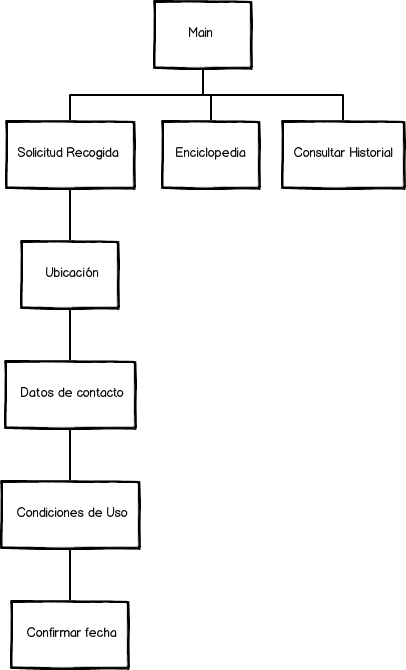
\includegraphics[scale=0.5]{Views.png} 
\caption{Esquema de vistas de la aplicación.}
\end{figure}	

A continuación se incluyen los diversos bocetos de las distintas pantallas de la aplicación móvil. 

% VISTA MENÚ PRINCIPAL
 \begin{figure}[H]
\centering
	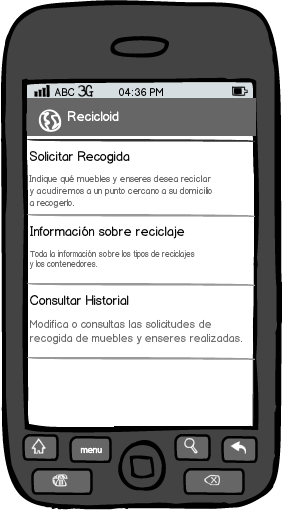
\includegraphics[scale=0.5]{MainLayout.png} 
\caption{Boceto del menú principal}
\end{figure}
Esta es la primera ventana que visualiza el usuario, se incluye el titulo de la aplicación acompañado de un pequeño icono que la identificará en todo momento. Debajo de esta una lista con las 3 opciones principales y cada una de ellas acompañadas de una breve descripción de en qué consiste cada una de ellas. Se incluye además una imagen que identifica visualmente cada opción para mayor comodidad del usuario. Este menú principal puede ir precedido de un \textit{splash} con la imagen de la organización encargaría de prestar el servicio. Una vez se haga \textit{click} sobre alguna de las tres opciones se abrirá la vista correspondiente. 
% VISTA SOLICITUD RECOGIDA
 \begin{figure}[H]
\centering
	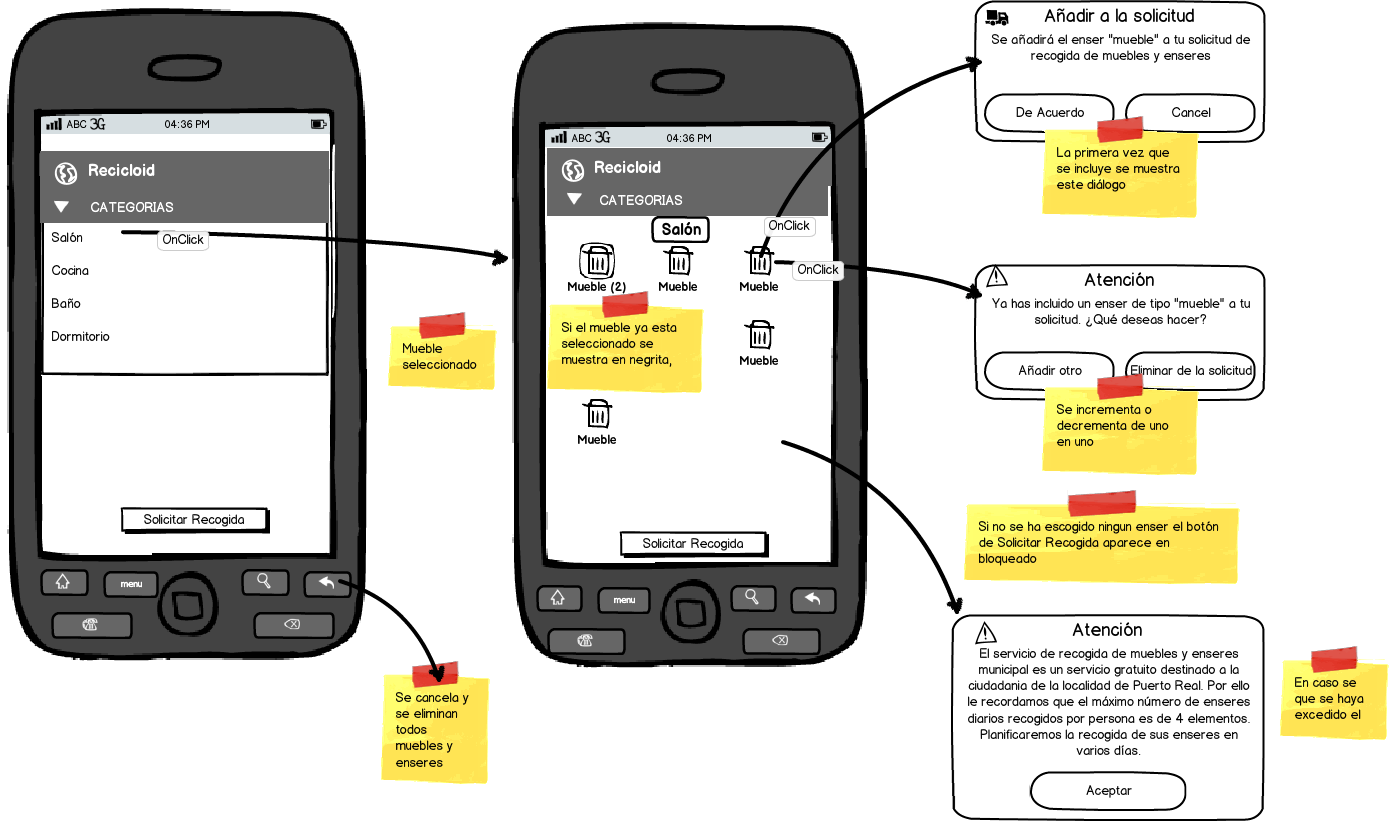
\includegraphics[scale=0.35]{SolicitudRecogidaLayout.png} 
\caption{Boceto de la solicitud de recogida}
\end{figure}
Una vez el usuario ha seleccionado la opción de solicitar recogida, se muestra un menú desplegable con todas las categorías existentes (Se categorizan los muebles y enseres en función de su ubicación). Una vez el usuario selecciona en el menú desplegable una habitación se muestra una ventana con pequeños iconos acompañados de texto con los distintos muebles y enseres que corresponden a dicha habitación. Cuando el usuario hace click en uno por primera vez se haber una ventana emergente en la cual se informa al usuario que dicho enser será añadido al listado de muebles y enseres de la solicitud, se pide confirmación o cancelación. Si el usuario indica que desea añadirlo éste queda resaltado y con el texto en negrita. Además el texto aparece acompañado con un paréntesis donde se indica la cantidad de enseres que se han seleccionado. \\
Si el usuario marca por segunda vez un icono de enser que ya ha sido previamente seleccionado aparece una nueva ventana emergente que posibilita incrementar el enser en uno, o bien eliminar todos los enseres de ese tipo de la solicitud. \\
En caso de que el usuario añada un cuarto enser a su solicitud se informa al usuario de que su petición se llevará a cabo en varios días, ya que el máximo diario establecido por usuario es de la recogida de 4 enseres al día. También se controla que el usuario no ejecuté solicitudes vacías demarcando el botón hasta que se escoja al menos un mueble y enser. En caso de que el usuario seleccione volver al menú principal se eliminan todos los iconos marcados y se deja como inicialmente encontraba. 
% UBICACIÓN
 \begin{figure}[H]
\centering
	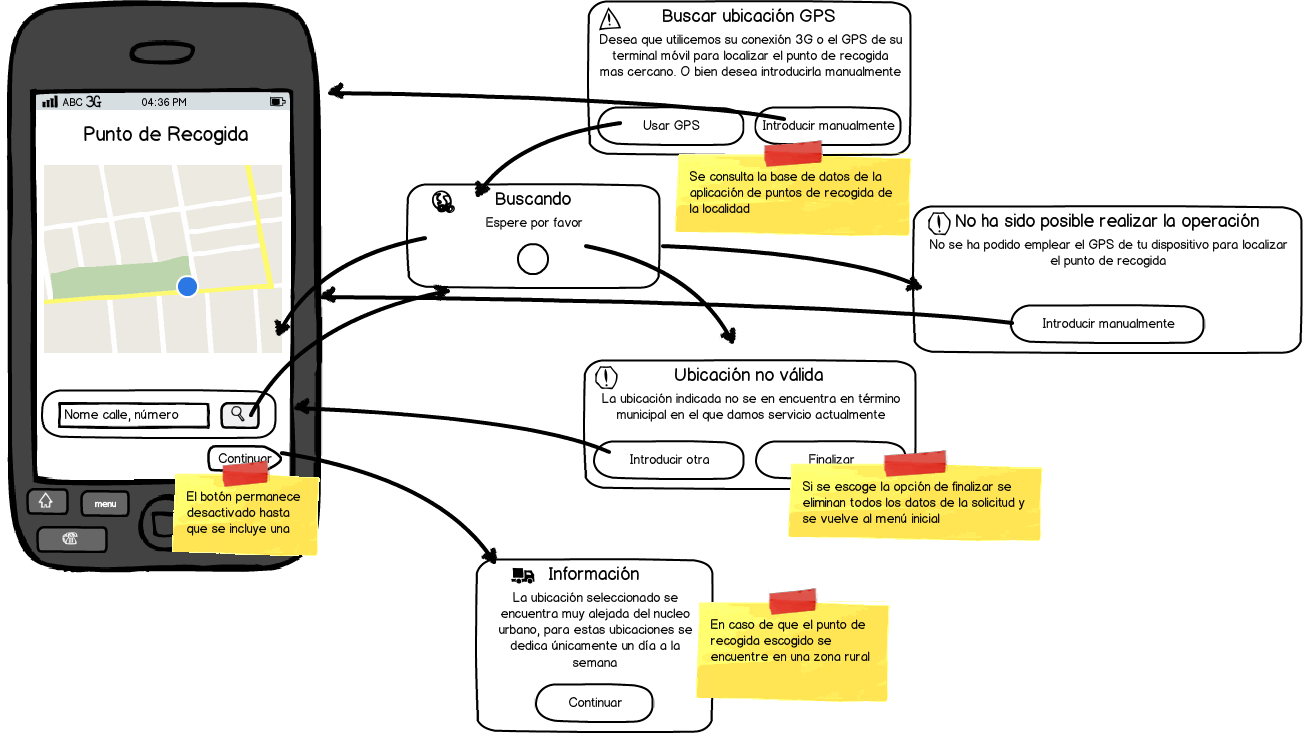
\includegraphics[scale=0.35]{SolicitudUbicacionLayout.png} 
\caption{Boceto de ubicación de la recogida}
\end{figure}
Se muestra una ventana al usuario preguntándole si desea que se localice el punto mas cercano del que se encuentra actualmente haciendo uso del dispositivo móvil, o bien si desea introducirla manualmente \\
En caso de escoger la opción de "Usar GPS" se hará uso de la tecnología existente en el terminal móvil para obtener la ubicación actual y seguidamente contrastarlo con la base de datos local del teléfono móvil con todos los puntos de recogidas existentes. Si se localiza correctamente se muestra en el mapa y se indica el nombre del a calle y el número más cercano. Puede ocurrir que la ubicación se encuentre fuera del termino municipal donde se preste servicio en cuyo caso se mostrará un mensaje informando de que la ubicación no es válida y posibilitando que introduzca manualmente una nueva ubicación. De igual manera, pude ocurrir que el dispositivo GPS no funcione correctamente en cuyo caso se informará del error y se indicará al usuario que introduzca manualmente la dirección. Durante la duración de la operación de búsqueda en el dispositivo GPS aparecerá una ventana de cargando con una animación y un mensaje solicitando al usuario su espera. Se establecerá un tiempo máximo de respuesta.  \\
Si el usuario escoge introducir manualmente su ubicación introducirá su calle y su número. Posteriormente el sistema detectará las coordenadas del domicilio del cliente y buscará la ubicación más cercana cotejando con la base de datos de puntos de recogida existente en el sistema. De igual manera puede darse el caso de que la ubicación no sea válida al encontrarse fuera del término municipal.  \\
Finalmente una vez obtenida la dirección del punto de recogida en el caso de que el punto de recogida esté alejado del término municipal se informa al usuario de las condiciones de uso existentes para esta tipología de usuarios.  \\
El botón para continuar con el proceso de solicitud de recogida de muebles y enseres no estará habilitado hasta que se haya escogido un punto de recogido válido. 

% DATOS DE CONTACTO
 \begin{figure}[H]
\centering
	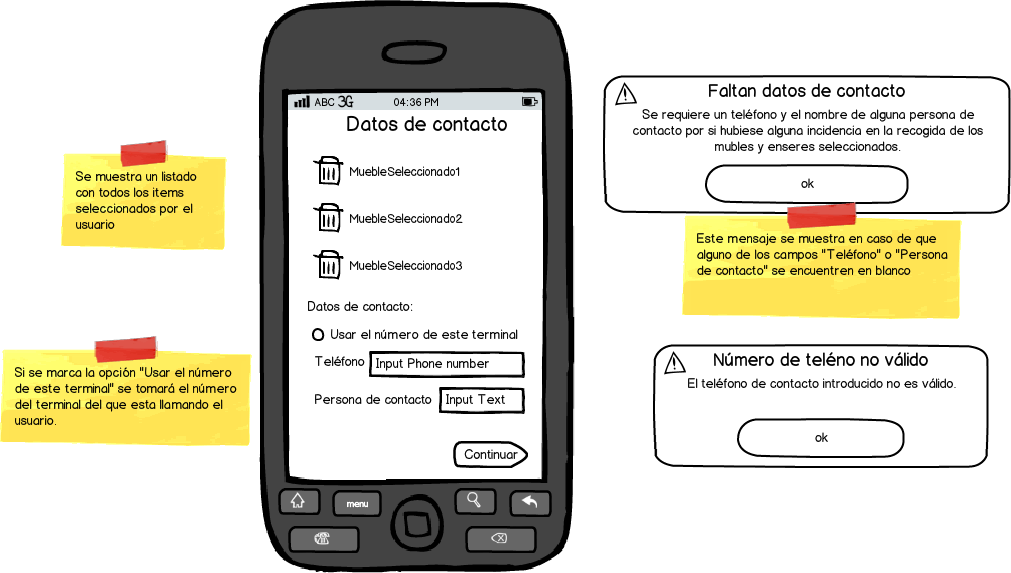
\includegraphics[scale=0.35]{SolicitudDatosContactoLayout.png} 
\caption{Boceto de datos de contacto}
\end{figure}
Se muestra una ventana en la que solicitan al usuario sus datos de contacto, en la parte superior a modo de recordatorio se incluye un listado de todos los enseres que ha solicitado el usuario que sean recogidos. Debajo de estos se muestra un formulario en el que se piden al usuario sus datos de contacto. Estos datos pueden ser introducidos manualmente por el usuario o bien ser tomados del propio terminal móvil. Se comprueba que el número de teléfono es correcto y que ambos cambios han sido rellenado correctamente antes de continuar con el proceso de tramitación de la solicitud. 

% CONDICIONES DE USO
 \begin{figure}[H]
\centering
	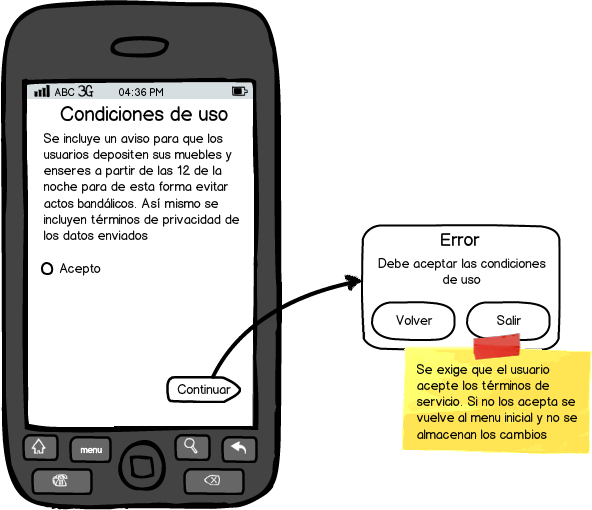
\includegraphics[scale=0.35]{SolicitudCondicionesLayout.png} 
\caption{Boceto de las condiciona de uso}
\end{figure}
Antes de finalizar el proceso y dado que los datos del usuario quedarán registrados en el servidor se muestra una ventana con las condiciones de uso y aspectos legales. Entre estas condiciones están las requeridas por la organización de informar a los usuarios de su responsabilidad de despistar los muebles y enseres a la hora mas tardía de la noche posible para evitar posibles actos vandálicos así como información referente al uso de sus datos por parte de la organización. El usuario debe aceptar las condiciones de uso para hacer uso del servicio.

% FECHA DE RECOGIDA
  \begin{figure}[H]
\centering
	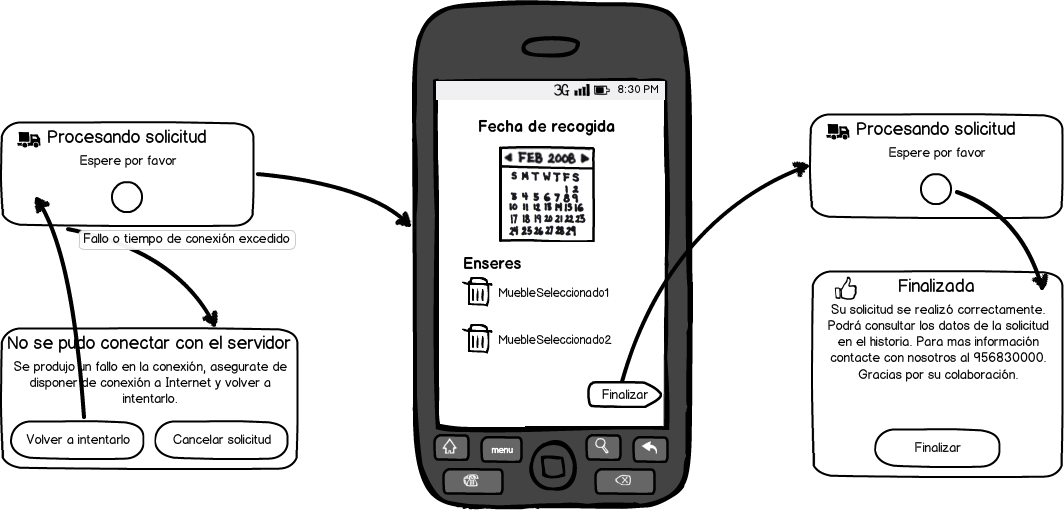
\includegraphics[scale=0.35]{SolicitudFechaLayout.png} 
\caption{Boceto de fecha de recogida}
\end{figure}
Se establece una conexión con el servidor para concertar la fecha de la recogida de muebles y enseres. En caso de producirse un error o de no tener habilitada la conexión se mostrará una ventana emergente con el error que se ha producido para que el usuario reintente la conexión o bien cancele el proceso. Una vez establecida la conexión se muestra un calendario con las fechas establecidas  y un recordatorio con los enseres que serán depositados. En el caso de ser mas de 4 enseres aparecerán varias fechas remarcadas en el calendario. Una vez el usuario confirma las fechas se establece una segunda conexión en la que se confirma la solicitud mediante un mensaje de agradecimiento ola usuario y un recordatorio del teléfono de contacto para cualquier duda posible. Finalizado el proceso se vuelve al menú principal. 

% ENCICLOPEDIA DE RECICLAJE
  \begin{figure}[H]
\centering
	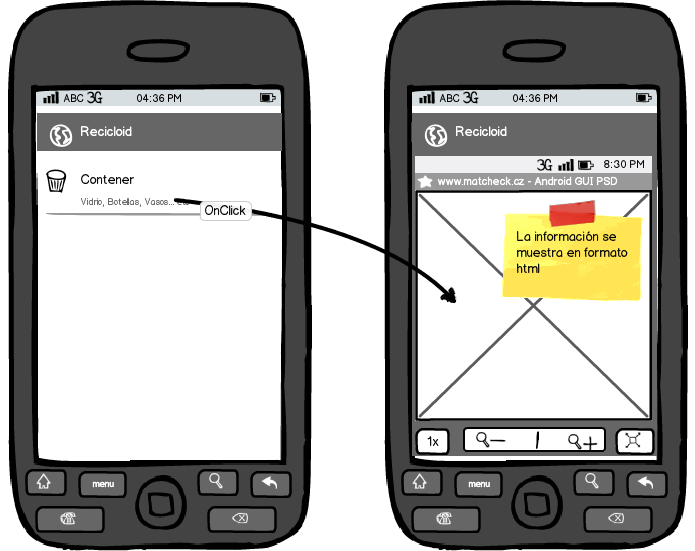
\includegraphics[scale=0.35]{EnciclopediaLayout.png} 
\caption{Boceto de guía de reciclaje}
\end{figure}
La aplicación incluye una guía de reciclaje en la que se muestran los distintos tipos de contenedores y un breve resumen del tipo de residuos que van depositados en dicho contenedor. Si el usuario marca alguno de los contenedores se abre el navegador web del usuario a una página en formato adaptado para terminales móviles con información sobre dicho tipo de contenedor un listado del tipo de residuos que van en dicho contenedor. Esta web funciona a modo local y no requiere de conexión a internet.

% HISTORIAL 
  \begin{figure}[H]
\centering
	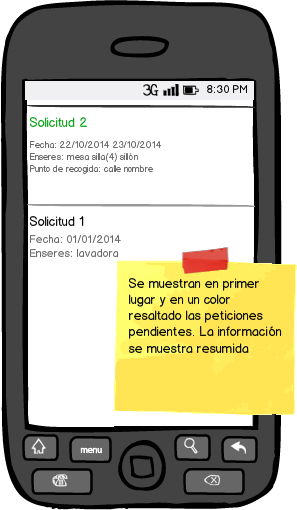
\includegraphics[scale=0.35]{HistorialSolicitud.png} 
\caption{Boceto de historial de solicitudes}
\end{figure}
La tercera de las opciones del menú principal es el \textit{Historial de solicitudes}. Mediante esta opción se muestra al usuario un listado resumido de las solicitudes que se han realizado. En primer lugar aparecerán resaltado en verde las que se han realizado para días posteriores a la fecha del sistema. Debajo de ésta aparecerán las peticiones cursadas anteriormente y cuya fecha de recogida ya ha transcurrido. \\

\newpage
\subsection{Diseño de datos}
% En esta sección se define la estructura física de datos que utilizará el sistema, a partir del modelo de conceptual de clases, de manera que teniendo presente los requisitos establecidos para el sistema de información y las particularidades del entorno tecnológico, se consiga un acceso eficiente de los datos. La estructura física se compone de tablas, índices, procedimientos almacenados, secuencias y otros elementos dependientes del SGBD a utilizar.
% Base de datos de la aplicación móvil
Se desea almacenar en el terminal móvil información referida a las solicitudes de recogida de muebles y enseres llevadas a cabo por el usuario de la aplicación, a fin de que este pueda consultarlas posteriormente las haya cursado. Dicha información sobre solicitudes incluirá información sobre las fechas (tanto de solicitud como de recogida), la ubicación donde acudirá el camión a recoger los enseres, y los enseres en si mismos que el usuario desea depositar. Dicha información además se empleará para poder gestionar el proceso de la solicitud de recogida de enseres permitiendo la clasificación de enseres en categorías y consultando todos los puntos de recogida de la localidad donde se preste servicio. \\
\begin{itemize}

\item \textbf{Enseres: }entre los enseres se incluyen tanto muebles como electrodomésticos de gran volumen que serán recogidos por el servicio de recogida y trasladados al punto limpio de la localidad. La organización desea información sobre los enseres para gestionar la recogida por parte del servicio de transporte. A cada enser en la aplicación móvil se le asociará un icono para mostrarlo al usuario. Los enseres serán identificados por un identificador único y contarán con un nombre.

\item \textbf{Punto de recogida: }representa los distintos puntos donde se depositan los muebles y enseres, Estos puntos coinciden con la ubicación de contenedores de otro tipo, y será la ubicación donde el camión llevará a cabo su parada para recoger dichos encere depositados previamente el usuario. De los puntos de recogida interesa conocer un identificador único, la localización en términos de latitud y longitud de cara a poder hacer uso de la tecnología gas del terminal móvil del usuario. Y como información aproximada la calle en la que se encuentre. Los puntos de recogida podrán ser de dos tipos: zonas cercanas al término municipal donde la recogida es diaria, y zonas alejadas del término municipal donde la recogida se realiza un día a la semana. Un punto de recogida tendrá un identificador numérico, y una localización que incluirá las coordenadas de longitud y latitud para su localización. Además del nombre de la calle en la que se encuentra. Aclarar que en una calle pueden existir varios puntos de recogida.

\item \textbf{Zona: }Se distingues a priori dos zonas distintas, las rurales y las urbanas. En las zonas urbanas la recogida se efectúa a día y para las zonas rurales hay un día para cada recogida. Podría ocurrir que en un futuro se incluyesen otras zonas. Las zonas vienen identificadas por una id y incluyen un nombre.

\item \textbf{Solicitudes de recogida: }toda solicitud de recogida incluye uno o varios enseres que serán recogidos en una o varias fechas. Además la solicitud va asociado un punto de recogida. La solicitud vendrá identificada por un valor numérico asociado a la solicitud llevada  a cabo por el usuario. Se incluirán dos fechas: por un lado la fecha de solicitud en la que el usuario contactó con el servicio de recogida de muebles y enseres y concertó la solicitud, y por otra parte la fecha de recogida asociadas a esa solicitud. 

\end{itemize}

\textbf{Restricciones semánticas} \
\
\begin{itemize}

\item Toda \textit{solicitud de recogida} tendrá de uno a cuatro {enseres} incluidos.

\item La \textit{fecha de solicitud} corresponderá al a fecha en la que se solicitó la recogida y la \textit{fecha de recogida} será posterior a esta y corresponderá a la fecha en la que se recogerán los muebles y enseres.

\item  La \textit{solicitud de recogida} se realizará en un único punto de recogida.

\item No existen dos \textit{puntos de recogida} con la misma \textit{localización}

\item No existen dos \textit{Zonas} con el mismo \textit{nombre}.

\end{itemize}

\textbf{Diagrama ER}

% Diagrama ER
\begin{figure}[H]
\centering
	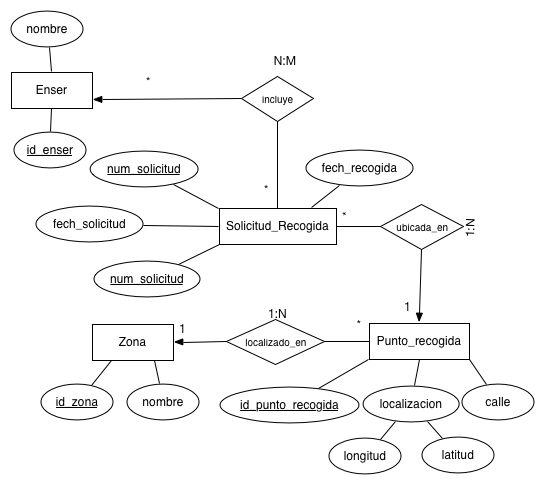
\includegraphics[scale=0.75]{bd-recicloid.png} 
  	 \caption{Diagrama ER de la base de datos de la aplicación móvil}
\end{figure}
 
\textbf{Zonas} \\
A la hora de diseñar las zonas, y dado que hay que distinguir entre zonas del núcleo urbano y las zonas rurales (campos y residencias alejadas del término municipal) se ha optado por realizar un acotamiento de zonas definiendo un polígono con los parámetros de latitud y longitud. De esta forma una vez se obtengan los datos de la posición donde se encuentra el usuario se procederá a comprobar si el usuario se encuentra en el término municipal y si esta es una zona urbana o si se encuentra alejado. Los datos se almacenarán en dos ficheros xml. A continuación se muestran los polígonos que se han definido para cada una de dichas zonas. 

% Acotamiento por coordenadas
\begin{figure}[H]
\centering
	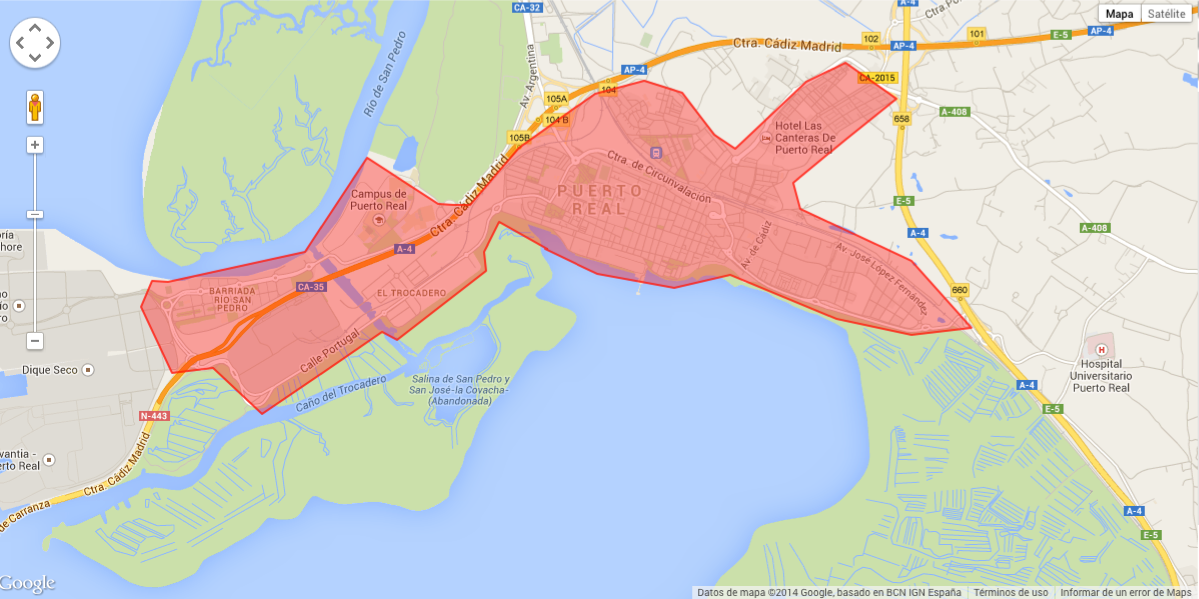
\includegraphics[scale=0.3]{zona-urbana.png} 
\caption{Acotamiento de mapa para la zona urbana del municipio.}
\end{figure}	

\begin{figure}[H]
\centering
	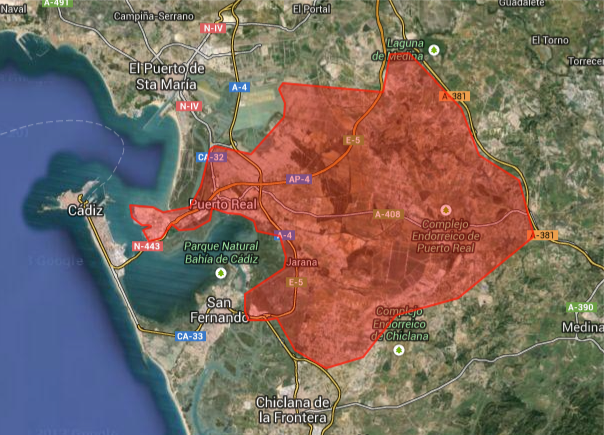
\includegraphics[scale=0.5]{termino-municipal.png} 
\caption{Acotamiento de mapa para la totalidad del municipio.}
\end{figure}

De este polígono se obtiene una serie de vértices con el formato ( \textbf{latitud} , \textbf{longitud} ) que serán cargados cuando el usuario desee establecer el puto de su domicilio al solicitar la recogida de muebles y enseres. De esta forma se puede averiguar cuando se obtenga una coordenada si se encuentra dentro de la zona de servicio y si corresponde a una zona urbana o no. El formato de los ficheros xml incluidos en la app móvil es el siguiente:

% Código en que se explica como se ha ellaborado el fichero xml con las ubicaciones
\begin{lstlisting}[style=XML]
<?xml version="1.0" encoding="UTF-8" ?>
<zone>
  <item>
    <latitude>36.48038014291644</latitude>
    <longitude> -6.178951263427734</longitude>
  </item>
  <item>
    <latitude>36.47085575451313</latitude>
    <longitude> -6.179466247558594</longitude>
  </item>
  ...
</zone>
\end{lstlisting}


\subsection{Diseño de componentes}
% En esta sección se definen los componentes software necesarios para la implementación del sistema. Es recomendable organizarlo en forma de subsistemas, a su vez de módulos. Estos módulos (o paquetes) contendrán un conjunto de artefactos software, que representaremos en forma de clases y que corresponderán a una de las capas identificadas en la arquitectura.
% Para cada uno de los módulos funcionales del sistema debemos realizar un diagrama de secuencia, para definir la interacción existente entre las clases de objetos que permitan responder a eventos externos. A partir de este diagrama, se genera el diagrama de clases de diseño, incluyendo los elementos del modelo conceptual, enriquecidos con las nuevas clases, relaciones, atributos y operaciones resultantes. Asimismo, se detallará el comportamiento de las operaciones más relevantes.

\subsection{Parametrización del software base}
% En esta sección, se detallan las modificaciones a realizar sobre el software base, que son requeridas para la correcta construcción del sistema. En esta sección incluiremos las actuaciones necesarias sobre la interfaz de administración del sistema, sobre el código fuente o sobre el modelo de datos.

\section{Implementación del Sistema}
\subsection{Entorno tecnológico}
	\section{Análisis de Requisitos}
\subsection{Catálogo de actores}
	\input{desarrollo/tablas/ACT-0001.tex}
	\input{desarrollo/tablas/ACT-0002.tex}
	
\subsection{Requisitos funcionales}
\subsubsection*{Casos de uso del sistema}
	\begin{figure}[H]
	\centering
 	   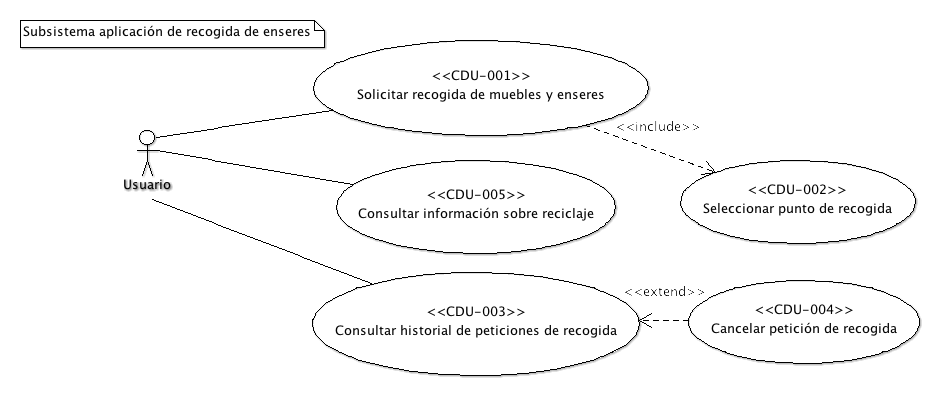
\includegraphics[scale=0.50]{diagramaCU1.png} 
  	  \caption{Diagrama UML del Subsistema aplicación de recogida de muebles y enseres.}
	\end{figure}	
	\input{desarrollo/casosDeUso/CDU-001.tex}
	\input{desarrollo/casosDeUso/CDU-002.tex}
	\input{desarrollo/casosDeUso/CDU-003.tex}	
	\input{desarrollo/casosDeUso/CDU-004.tex}
	\input{desarrollo/casosDeUso/CDU-005.tex}	
	
	\begin{figure}[H]
	\centering
 	   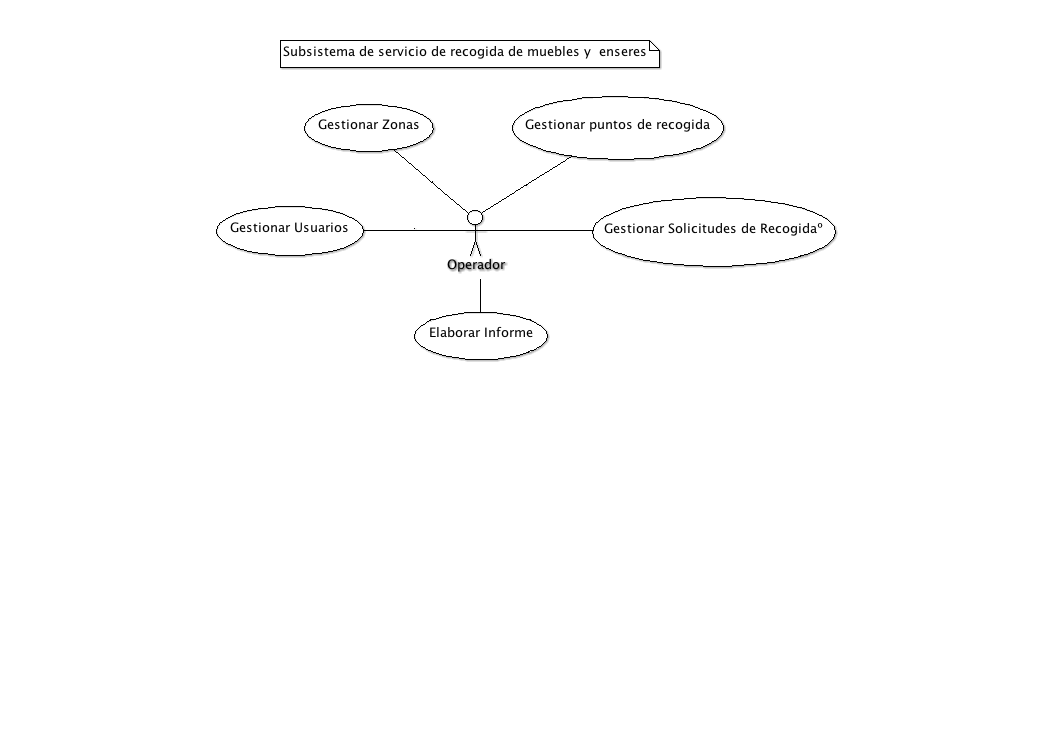
\includegraphics[scale=0.50]{diagramaCU2.png} 
  	  \caption{Diagrama UML del Subsistema de servicio de recogida de muebles y enseres.}
	\end{figure}	

\subsection{Requisitos de información}
	\input{desarrollo/tablas/IRQ-0001.tex}
	\input{desarrollo/tablas/CRQ-001.tex}
	\input{desarrollo/tablas/IRQ-0002.tex}
	\input{desarrollo/tablas/CRQ-002.tex}	
	\input{desarrollo/tablas/IRQ-0003.tex}
	\input{desarrollo/tablas/CRQ-003.tex}	
	\input{desarrollo/tablas/IRQ-0004.tex}
	
	\newpage
	\subsubsection*{Diagrama conceptual de clases UML}
	\begin{figure}[H]
	\centering
 	   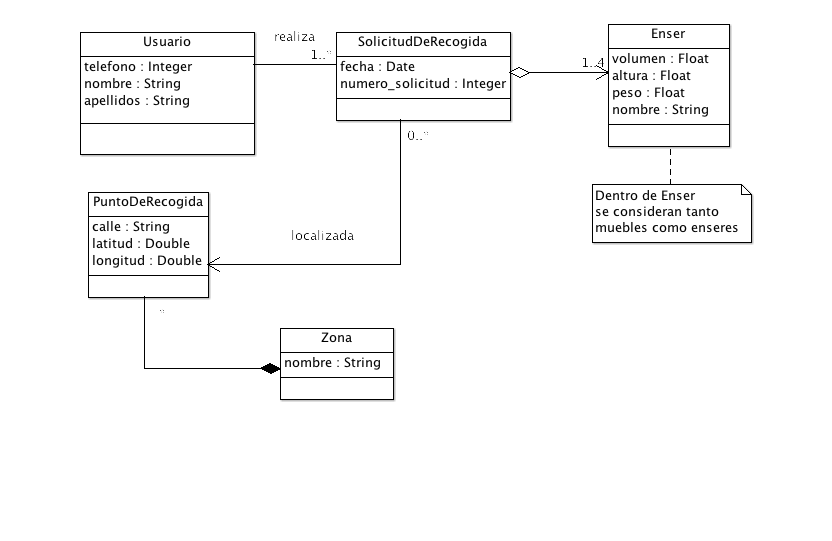
\includegraphics[scale=0.70,angle =90]{diaConceptualUML.png} 
  	  \caption{Diagrama conceptual de clases UML.}
	\end{figure}
	
	\newpage
	\subsubsection*{Tipos}
	% Tipo Usuario
	\input{desarrollo/clases/TYP-001.tex}
	% Tipo SolicitudRecogida	
	\input{desarrollo/clases/TYP-002.tex}	
	% Tipo PuntosDeRecogida	
	\input{desarrollo/clases/TYP-003.tex}		
	% Tipo Zonas	
	\input{desarrollo/clases/TYP-004.tex}
	% Tipo Enseres	
	\input{desarrollo/clases/TYP-005.tex}	
				
\subsection{Requisitos no funcionales}
% Descripción de otros requisitos (relacionados con la calidad del software) portabilidad, seguridad, auditoría, monitorización, fiabilidad,
% comunicaciones con sistemas externos, extensibilidad, rendimiento, escalabilidad, estándares de obligado cumplimiento, accesibilidad, usabilidad, aspectos de la interfaz de usuario, 
% utilización de un determinado entorno tecnológico, etc.
\subsubsection*{Seguridad}
El servidor donde se almacenarán y procesarán las solicitudes de los usuarios se encuentra ubicado en la Intranet del ayuntamiento. Por seguridad no se debe permitir el acceso directo de la app móvil al servidor, por lo que se hace imprescindible que un servicio se encargue de intermediar entre el servidor y la aplicación del usuario, así como gestionar las diversas peticiones. En todo momento es de vital importancia controlar el aspecto de seguridad en las comunicaciones y conexiones que se establezcan. 

\subsubsection*{Interfaz}
Para poder maximizar el número de descargas de la aplicación y captar una mayor atención se debe cuidar el aspecto estético. La aplicación que se ofrecerá a la ciudadanía no solo debe ser visualmente atractiva sino identificarse con la empresa y la actividad que realiza. Así mismo, la información debe presentarse de una forma resumida y siempre que sea posible acompañada de un apoyo visual por medio de imágenes o iconografía.

\subsubsection{Usabilidad}
Se pretende hacer más cómoda  y fácil de realizar una gestión rutinaria como es la notificación de recogida de enseres. Es por ello importante que la aplicación sea sencilla de utilizar, y no presente ningún reto ni dificultad en su maneja. Se espere llegar a usuarios de toda edad y nivel formativo. 

\subsection{Reglas de negocio}
	\input{desarrollo/reglas-negocio.tex}	

\subsection{Estudio de alternativas tecnológicas}
% En esta sección, se debe ofrecer un estudio del arte de las diferentes alternativas tecnológicas que permitan satisfacer los requerimientos del sistema, para luego seleccionar la herramienta o conjunto de herramientas que utilizaremos como base para el software a desarrollar.

\subsection{Análisis GAP}
% Una vez seleccionado el software de base, debemos identificar y medir las diferencias entre lo que proporciona este software y los requisitos definidos
% para el proyecto. El resultado de este análisis permitirá identificar cuáles de éstos requisitos ya están solventados total o parcialmente por el sistema base y cuales tendremos que diseñar e implementar.

\section{Diseño del Sistema}	
\subsection{Diseño de la arquitectura}


\subsubsection{Arquitectura física}
% En este apartado, describimos los principales componentes hardware que forman la arquitectura física de nuestro sistema, recogiendo por un lado los componentes de servidor y los componentes de sistemas externos con los que colabora nuestro sistema y por otro, los componentes hardware de cliente.

\subsubsection{Arquitectura lógica}
% La arquitectura lógica del sistema está formada por los elementos software (servicios, aplicaciones, librerías, frameworks, etc.) que componen el
% software base, más el software desarrollado para cumplir los requisitos de la aplicación. También, se recogen los componentes de sistemas externos con los que interactúa nuestro sistema, así como los componentes software del lado cliente.


\subsubsection{Arquitectura de diseño}
% La arquitectura de diseño especifica la forma en que los artefactos software de más bajo nivel, interactúan entre sí para lograr el
% comportamiento deseado en el sistema. Utilizaremos el patrón arquitectónico Layers (Capas), con el cual estructuramos el sistema en un número apropiado de capas, de forma que todos los componentes de una misma capa trabajan en el mismo nivel de abstracción y los servicios proporcionados por la capa superior utilizan internamente los servicios proporcionados por la capa inmediatamente inferior.
%\textbf*{Capa de presentación} \\
%\textbf*{Capa de negocio} \\
%\textbf*{Capa de integración} \\
%\textbf*{Servicios trasversales} \\

\newpage
\subsection{Diseño de interfaz de usuario}
% En esta sección se especifican las interfaces entre el sistema y el usuario, detallando el aspecto y el comportamiento de las diferentes pantallas e informes, de acuerdo con el entorno tecnológico definido. Con respecto a las pantallas e informes, es preciso realizar un prototipo o mockup gráfico. Junto a estos bocetos hay que definir qué ocurre en los distintos componentes visuales de la interfaz cuando aparecen y qué acciones se disparan cuando el usuario trabaja con ellas.
% Además, es preciso elaborar un diagrama de navegación, reflejando la secuencia de pantallas a las que tienen acceso los diferentes roles de usuario y la conexión entre éstas.
\input{desarrollo/disenoUI.tex}

\newpage
\subsection{Diseño de datos}
% En esta sección se define la estructura física de datos que utilizará el sistema, a partir del modelo de conceptual de clases, de manera que teniendo presente los requisitos establecidos para el sistema de información y las particularidades del entorno tecnológico, se consiga un acceso eficiente de los datos. La estructura física se compone de tablas, índices, procedimientos almacenados, secuencias y otros elementos dependientes del SGBD a utilizar.
\input{desarrollo/dis-datos.tex} 
\input{desarrollo/dis-zonas.tex}

\subsection{Diseño de componentes}
% En esta sección se definen los componentes software necesarios para la implementación del sistema. Es recomendable organizarlo en forma de subsistemas, a su vez de módulos. Estos módulos (o paquetes) contendrán un conjunto de artefactos software, que representaremos en forma de clases y que corresponderán a una de las capas identificadas en la arquitectura.
% Para cada uno de los módulos funcionales del sistema debemos realizar un diagrama de secuencia, para definir la interacción existente entre las clases de objetos que permitan responder a eventos externos. A partir de este diagrama, se genera el diagrama de clases de diseño, incluyendo los elementos del modelo conceptual, enriquecidos con las nuevas clases, relaciones, atributos y operaciones resultantes. Asimismo, se detallará el comportamiento de las operaciones más relevantes.

\subsection{Parametrización del software base}
% En esta sección, se detallan las modificaciones a realizar sobre el software base, que son requeridas para la correcta construcción del sistema. En esta sección incluiremos las actuaciones necesarias sobre la interfaz de administración del sistema, sobre el código fuente o sobre el modelo de datos.

\section{Implementación del Sistema}
\subsection{Entorno tecnológico}
	\section{Análisis de Requisitos}
\input{desarrollo/analisisDeRequisitos.tex}

\section{Diseño del Sistema}	
\input{desarrollo/disenoDelSistema.tex}

\section{Implementación del Sistema}
\subsection{Entorno tecnológico}
	\input{desarrollo/entorno-tecnologico/index.tex}
	
\subsection{Código fuente}

\subsection{Calidad del código}

\section{Pruebas del Sistema}

\subsection{Pruebas unitarias}

\subsection{Pruebas de integración}

\subsection{Pruebas del sistema}

\subsubsection{Pruebas funcionales}

\subsubsection{Pruebas no funcionales}

\subsection{Pruebas de aceptación}

	
\subsection{Código fuente}

\subsection{Calidad del código}

\section{Pruebas del Sistema}

\subsection{Pruebas unitarias}

\subsection{Pruebas de integración}

\subsection{Pruebas del sistema}

\subsubsection{Pruebas funcionales}

\subsubsection{Pruebas no funcionales}

\subsection{Pruebas de aceptación}

	
\subsection{Código fuente}

\subsection{Calidad del código}

\section{Pruebas del Sistema}

\subsection{Pruebas unitarias}

\subsection{Pruebas de integración}

\subsection{Pruebas del sistema}

\subsubsection{Pruebas funcionales}

\subsubsection{Pruebas no funcionales}

\subsection{Pruebas de aceptación}


%\chapter{Epilogo}
%\part{Epilogo}
\section{Manual de usuario}
\subsection{Introducción}
\subsection{Características}
\subsection{Requisitos previos}
\subsection{Utilización}
\section{Manual de instalación y explotación}
\subsection{Introducción}
\subsection{Requisitos previos}
\subsection{Inventario de componentes}
\subsection{Procedimientos de instalación}
\subsection{Procedimientos de operación y nivel de servicio}
\subsection{Pruebas de implantación}
\section{Conclusiones}
\subsection{Objetivos}
\subsection{Lecciones aprendidas}
\subsection{Trabajo futuro}

\backmatter % Apéndices, bibliografía ...

\clearpage
\addcontentsline{toc}{chapter}{Bibliografia y referencias}
\chapter*{Bibliografia y referencias}
\nocite{*}
\printbibliography[heading=none]
\newpage

% Glosario
\addcontentsline{toc}{chapter}{Glosario}
\chapter*{Glosario}
\input{glosario.tex}

% Anexos
\addcontentsline{toc}{chapter}{Anexos}
\chapter*{Anexos}
\subsection*{Boceto inicial}
\begin{figure}[H]
\centering
    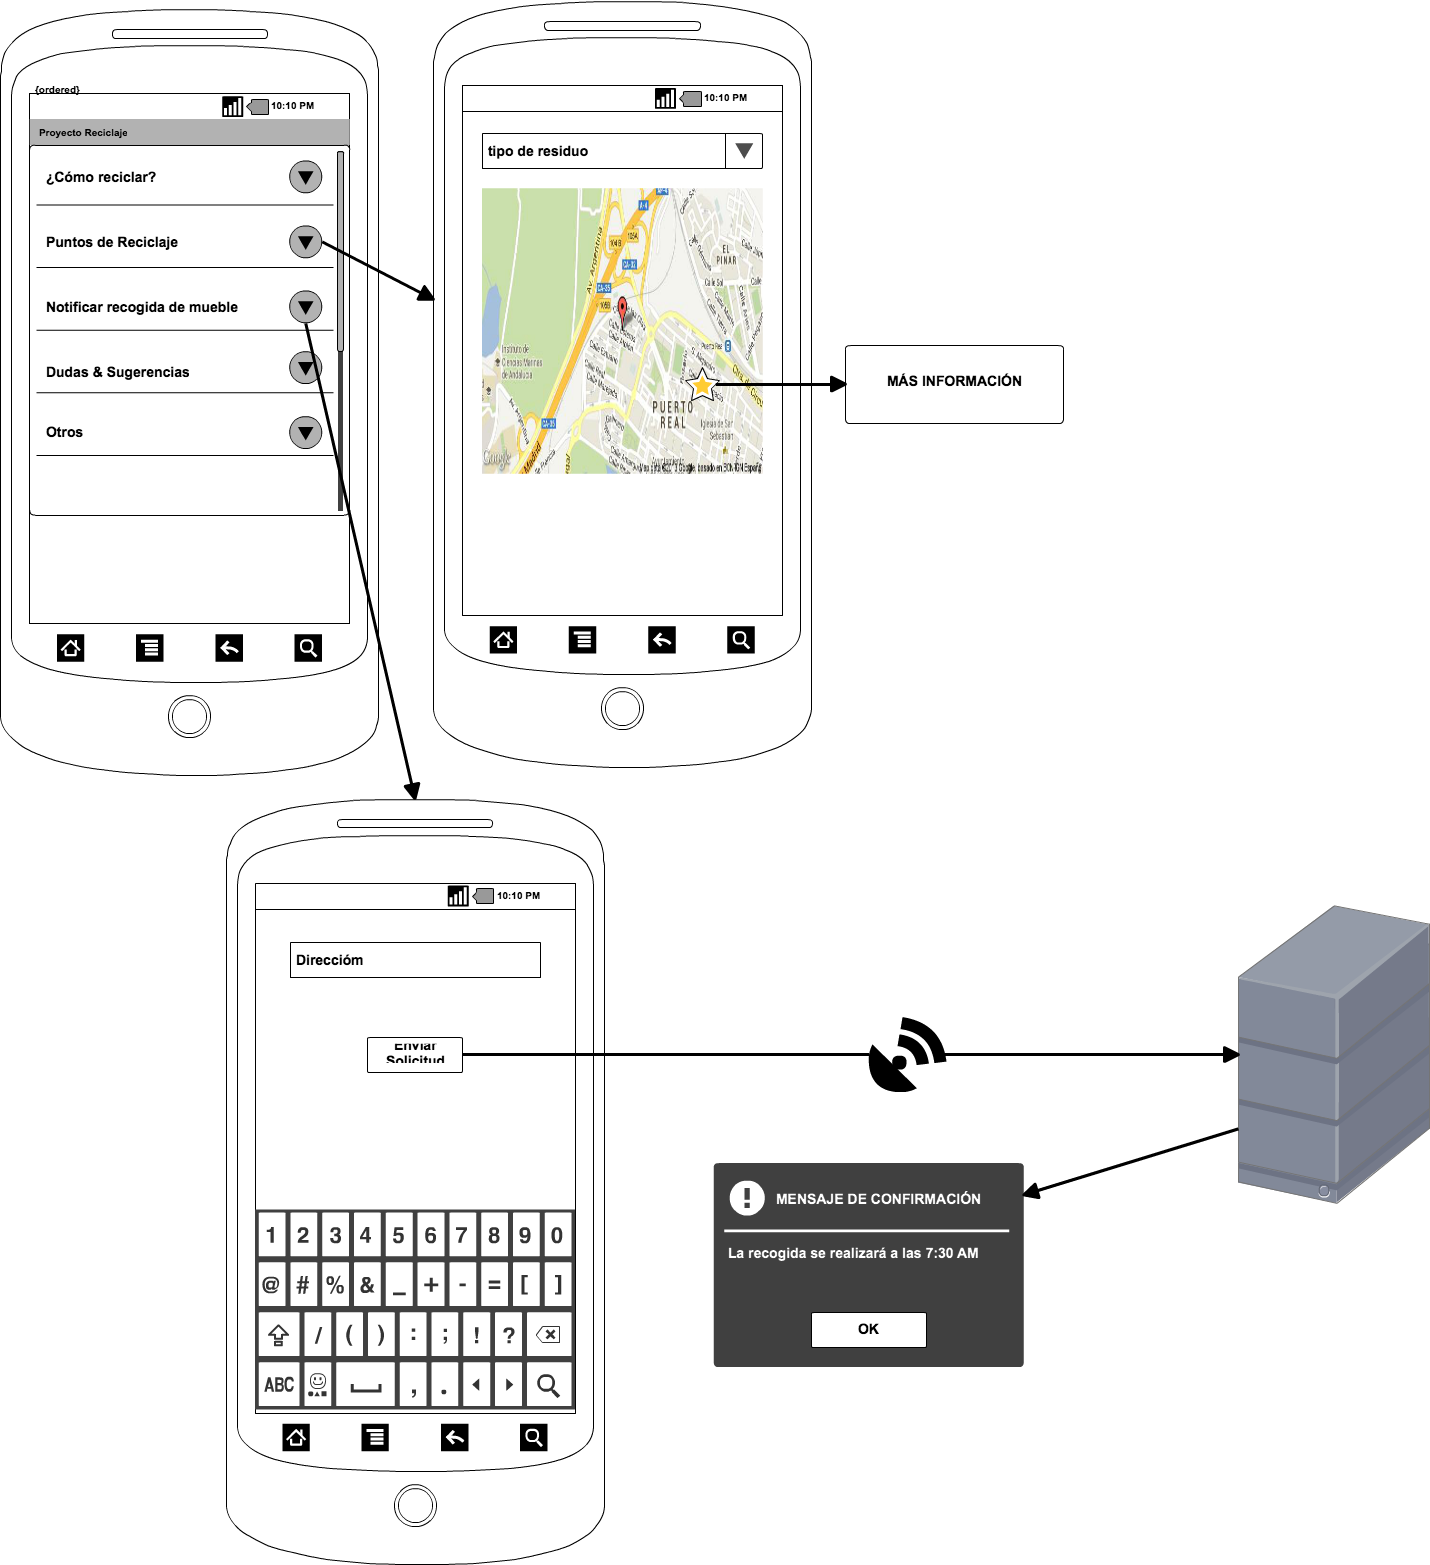
\includegraphics[scale=0.25]{boceto.png} 
    \caption{Boceto inicial}
\end{figure}
\newpage
\subsection*{Entrevista de elicitación}
Se incluye a continuación un resumen de la entrevista realizada el día 3 de diciembre de 2013 a los principales responsables del Área Informática del Ayuntamiento de Puerto Real y del Servicio de Recogida de Enseres y Limpieza. En ella nos encontramos presentes los siguientes participantes:
\begin{itemize}
\item Diego Rubio Abujas (entrevistador e ingeniero de requisitos).
\item Enrique Daneri (analista de sistema actual y responsable de la parte de aplicaciones).
\item Javier (actual responsable de la operativa de gestión de recogida de enseres).
\end{itemize}
 
La entrevista se inicia solicitando a los participantes su consentimiento para realizar la grabación de dicha entrevista. Se expone como motivo inicial de la entrevista, conocer el funcionamiento interno de la organización.
 
% EL PROCEDIMIENTO A SEGUIR
 
% Intervención del analista.
\paragraph{Enrique} Aunque dice no ser el responsable de la operativa, nos explica que se realizan una media de 20 recogidas diarias como máximo.  Nos comenta además que se realizan recogidas todos los días laborables. Es un solo camión el que realiza las recogidas actualmente. El proceso consiste en que el usuario realiza una llamada, el operador que recibe la llamada y tiene acceso a un registro de contenedores y actuales recogidas concertadas. El operador indica al usuario dónde debe depositar el elemento.  
\paragraph{} El proceso se realiza de la siguiente manera: hay una llamada del usuario y una vez recibida se le indica cuando debe depositar el mueble o el elemento a recoger. Si la fecha de recogida se prolonga más de 2 días, se ponen en contacto con el usuario para confirmar la recogida. 

\paragraph{}El analista nos da su punto de vista sobre la aplicación. La tecnología existente es efectuar una llamada a un operador y este proporciona la cita. Una forma de plantear la cita es indicar quien la solicita y que sea un operador el que la confirme. Hay un límite de muebles a recoger (3 muebles aproximadamente). Si se identifica el domicilio, la aplicación podía indicar las formas más próximas al domicilio del cliente. Se define dónde quiere el usuario que se recojan sus muebles, se queda a la espera de que se procese su solicitud, y finalmente se le da respuesta. 
 
\paragraph{}Otra opción que nos proporciona Enrique es: que la gestión se realice  de forma automatizada. Nos recuerda que se recogen enseres 20 diarios. Se comprueba que lo que solicita el usuario está dentro de los límites establecidos, se  indica la fecha en la que debe depositar los enseres al usuario. Se da opción de que el usuario solicite una fecha concreta. Una vez procesada la petición, el sistema da respuesta al usuario. Cuando llega el día de recogida, la aplicación podría enviar al usuario un recordatorio. Ocurre a veces que el mueble no se encuentre en el punto de recogida porque alguien haya pasado por el punto de recogida y se lo haya llevado. 
 
% Intervención del responsable de operativa.
\paragraph{Javier} Nos explica que hay una casuística muy grande tanto en tipos de muebles como en el incidencias ocurridas. Nos muestra su desacuerdo en automatizar el proceso de recogida. Nos expone diversos ejemplos: incrementos en el número de muebles por la suma de peticiones de recogidas no notificadas de los diversos vecinos del usuario, la problemática de no dejar los muebles en el lugar indicado, las negativas de los clientes a adaptarse al procedimiento de recogida (tanto en horario como en ubicación), etc. Finalmente nos expone que pocos usuarios realizan la gestión por vía telefónica (ya sea por desconocimiento del número o de la operativa a seguir), se expone la opción de ofrecer una idea alternativa para realizar la gestión mediante el lanzamiento de una aplicación móvil. Nos expone que el proceso no tiene ninguna problemática, la problemática está en la ejecución de la operativa y eso se escapa de la aplicación al ser por muchísimos factores humanos. El problema es de logística interna.
 
% Intervención del analista,
\paragraph{Enrique} Recalca que no es problema de la aplicación sino de logística interna. La dificultad está en la recogida, en cerrar el proceso.
 
% Intervención del responsable de operativa.
\paragraph{Javier} El usuario llama con el móvil y pide la cita, y la parte teórica no tiene problemas. Según él, el problema es cerrar el proceso, incluso con el método actual el operador tiene problemas en cerrar el trámite, en cerrar el procedimiento. Nos comenta que, en un porcentaje bastante alto, hay complicaciones en el cierre de procedimiento, e incluso a día de hoy, surgen casuísticas nuevas de problemas al cerrar el procedimiento. Nos expone varios ejemplos de sucesos ocurridos:
\begin{itemize}
\item Un usuario deja un frigorífico a recoger en un punto. Cuando pasa el camión, no lo ve debido a que el frigorífico ha sido desmontado y despiezado por terceras personas y deben ponerse en contacto con el usuario para confirmar si ha depositado el frigorífico en el punto de recogida o no.
\item El usuario dice que va a dejar un frigorífico y luego deja un sofá.
\end{itemize}
Como alternativa, muestra su interés en el uso de una aplicación para facilitar el proceso. Se expone nuestra intención de ofrecer este servicio como una alternativa más a la gestión de tramitación de recogida de muebles. Javier muestra interés en realizar el cierre con un operador.
 
% Intervención del analista.
\paragraph{Enrique} Explica que el proceso, tal y como está ahora mismo, debería realizarse automatizado pero excluyendo las incidencias y que éstas sean realizadas por un operador en oficina.
 
% Intervención del responsable de operativa.
\paragraph{Javier} Insiste en que el cierre debe ser realizado por un operador en una oficina, y la respuesta enviada al usuario que haya solicitado la recogida del mueble.
 
% Intervención del entrevistador
\paragraph{Diego} Se explica de nuevo en qué consistiría la aplicación. Ésta recibiría las peticiones del usuario, seguidamente el operador verificaría las peticiones con incidencias y tramitaría las respuestas a cada uno de los usuarios. Se expone el tema de las incidencias y qué es lo que se hace en estos casos.
 
% INCIDENCIAS
% Intervención del responsable de operativa
\paragraph{Javier} En caso de incidencias, se contacta con el cliente por llamada telefónica. Las incidencias suelen terminar con una llamada. Como ejemplo, nos expone el caso de un conductor del camión de recogida de muebles que se encontró con un mueble dentro de un portal y después de intentar hablar con vecinos, fue imposible la recogida, y contactó con la central. Seguidamente la incidencia se solventó mediante una llamada al usuario que solicitó la recogida. En la oficina se dió la incidencia y en la oficina llamaron al teléfono de contacto para solucionar la incidencia. Otro de los casos que suelen ocurrir es cuando hay mas muebles de los que debería haber en el lugar de recogida. En dicho caso, también se contacta con el usuario y se trata de aclarar cuál es el mueble que se solicita recoger. Muchas incidencias son resueltas por los operarios del camión y otras deben ser resueltas desde la oficina. Se recalca que el procedimiento es simple pero el problema es la ejecución, sobretodo la afección al procedimiento por variables que no están dentro del mismo, como las variables humanas. Si en el procedimiento se mete una variable que no ha llamado por teléfono, se rompe el flujo del procedimiento.
 
% Intervención del analista,18.24
\paragraph{Enrique} El objetivo de la aplicación debe ser realizar la petición y que el sistema la confirme. El ejemplo más cercano es el sistema de petición de citas médicas. El usuario debe poder solicitar una cita médica y si no la desea, poder cancelarla. La confirmación debe incluir en qué día y en qué lugar estará el mueble para que lo recojan.
 
% Intervención del responsable de operativa
\paragraph{Javier} Es importante dejar claro a los usuarios en qué consiste el servicio y qué tipo de productos se aplica. La aplicación debe reconocer cuando algún elemento no entre dentro de los parámetros del servicio y apartarlo del procedimiento.
 
% Intervención del entrevistador
\paragraph{Diego} Se sugiere la opción de incluir información sobre reciclaje y puntos limpios.
 
% Intervención del responsable de operativa
\paragraph{Javier} El mapa va a ser un poco pobre ya que sólo hay punto limpio, pero se podrían incluir puntos dentro de la provincia. Hablando del \textit{punto limpio} surge una temática relacionada con objetos que no son muebles y deberían llevarse al \textit{punto limpio}. Entre tales objetos se incluyen electrodomésticos o aparatos eléctricos cuya envergadura y dimensiones hacen imposible que el ciudadano corriente pueda trasladarlos al punto limpio. En estos casos, el servicio de recogida de muebles coopera realizando dicho traslado. Entre estos utensilios se incluyen los utensilios de gran volumen como un frigorífico o una lavadora.  Incluir un tutorial sería necesario y una buena idea pero debe ser un tutorial escueto y sencillo, para evitar abrumar al usuario y directamente hacer que deje el utensilio en la calle sin realizar aviso. \\ Según nos informa, el pasado año, el porcentaje de muebles recogidos sin aviso estuvo en torno al 70\% del total, por lo que fomentar la notificación de recogidas tal vez sea un buen aporte.
 
% Intervención del entrevistador
\paragraph{Diego} Se plantea el tema de la recogida y almacenamiento de datos referentes al proceso de solicitud de recogida de enseres. También se plantea si hay algún interés en realizar estudios estadísticos sobre dichos datos.
 
% Intervención del analista,28.58
\paragraph{Enrique} En la petición se identifica qué enseres se deben recoger y un teléfono de contacto, además de concretar con el operador el sitio de recogida. Esta información se clasifica por zonas del término municipal de Puerto Real (que son unas 6 o 7 zonas) y se almacena. Mensualmente se realizan estudios estadísticos. Este servicio de recogida es un servicio encomendado por el Ayuntamiento y mensualmente se le manda un informe con este tipo de estadísticas. Dicho estudio incluye recogidas por petición propia, recogidas ajenas que no se han notificado y recogidas notificadas por los propios operarios.  Entre estas últimas, como ejemplo, se expone un servicio de recogida de vidrios que ve un sofá y lo notifica a la oficina para que se incluya en la gestión de recogida de muebles. Se identifica la vía de entrada de la petición (si es interna, externa, telefónica, etc.) \\  La aplicación que está actualmente en producción tiene un modulo de voz que estuvo en el portal del Ayuntamiento pero que no llegó a implantarse. Dicha aplicación redirigía las peticiones a la web y era el operador quien gestionaba la recogida de enseres. \\ Hay que tener en cuenta que el servicio es gratuito y quien llama no suele identificarse o dar sus datos completamente. El NIF se podría poner como dato opcional. El perfil podría ir identificado por el teléfono, el nombre, la fecha y el punto de recogida.
 
% Intervención del entrevistador
\paragraph{Diego} En referencia a los enseres, se pregunta qué información se pide al usuario que solicita la recogida (tamaño, volumen...)
 
 
% Intervención del responsable de operativa
\paragraph{Javier} Dice que si nos ponemos a clasificar los enseres no terminaríamos nunca. El número de enseres por cliente está entre 2 y 4, cómo máximo, debido a que la filosofía de base del servicio es que es un servicio público, no un servicio de mudanzas. Un servicio público tiene sus limitaciones y debe atender al máximo número de personas. Muchos usuarios piden cita para varios días, por lo que hay gente que entiende la función del servicio y gente que no.\\ La tipología es más bien genérica, porque te encuentras diversos tipos de tablas sueltas, muebles de cocina, mesitas de noche, etc. Lo que interesa, a efectos del servicio, es la cantidad y el volumen del objeto.
 
% Intervención del analista,28.58
\paragraph{Enrique} Es más fácil que el usuario describa lo que quiere y en la oficina, cuando le van a confirmar la cita, se lo clasifiquen.
 
% Intervención del responsable de operativa
\paragraph{Javier} En el peor de los casos, no se confirma.
 
% Intervención del entrevistador
\paragraph{Diego} Se expone que debe de haber más \textit{feedback} entre usuario y operador del servicio.
 
% Intervención del analista
\paragraph{Enrique} No es lo mismo que el usuario indique \textit{sofá}, que especifique que es un  \textit{sofá 3 plazas}. En la oficina reciben la petición y la confirman. Debe haber la posibilidad de que el usuario y la oficina se comuniquen en un mismo nivel. Puede darse el caso de que haya una petición para recoger 4 objetos y luego solo puedan recogerse 2, ya que se sale de las especificaciones dadas, o podría darse que el servicio ya estuviese completo y por diferentes razones, tuviese que recoger dos muebles un día y dos, otro día. Son muchos matices los que se debe  indicar al usuario para que se realice el servicio de una manera u otra.
 
% Intervención del entrevistador
\paragraph{Diego} Se comenta que, si la petición es muy compleja, se redirija al usuario a que efectúe la petición por vía telefónica con un operador.
 
% Intervención del analista,35.15
\paragraph{Enrique} Existe la opción de rechazar lo que pide el usuario. Por ejemplo, si el usuario solicita \textit{Quiero que me recojan una cocina} se le debería de mandar una respuesta denegando la petición y explicándole los motivos \textit{Si quiere que se le recoja la cocina, se le pueden concertar varias citas en función del volumen de muebles}. Existe el caso simple: \textit{Tengo un sofá, toma, lo recojo, fin de la operación}; y se deben considerar todas las posibilidades: que la aplicación tenga una recogida parcial, que se deniegue la recogida, etc. Si se incluye en la respuesta un campo de observaciones, se solucionaría el tema de la recogida parcial para que se le explique al usuario el por qué del rechazo de una petición, por ejemplo.

% Intervención del entrevistador 36.20
\paragraph{Diego} Se sugiere incluir una clasificación de peticiones automatizada, es decir, que las más completas las realice el operador y las más simples las realice el sistema.
 
% Intervención del analista,36.38
\paragraph{Enrique} Hay que proporcionar al usuario un formulario sencillo. El móvil nos identifica con el número, diciendo nombre y lugar de residencia. A continuación, la aplicación nos da una respuesta con una fecha, hora y lugar donde depositar los enseres. En resumen \textit{Yo vivo aquí y quiero que me recojáis esto}, seguidamente desde la oficina te dan la respuesta aceptando o denegando la petición. Un ejemplo de respuesta afirmativa sería \textit{Día 4 a las 8 de la mañana en este punto de recogida}.
 
% Intervención del responsable de operativa
\paragraph{Javier} Adicionalmente, hay que considerar más aspectos. Hay veces en que el usuario deposita los enseres después de la hora de recogida, es decir, una vez que el camión ya ha pasado. La casuística es inmensamente grande. Además, hay otros problemas, como ocurre en el caso de los muebles de gran volumen (por ejemplo, un colchón), y es que han sucedido diversos actos vandálicos (como incendios provocados a los enseres depositados), entonces, por sistema, se debería de informar al usuario de que bajo ningún concepto deje los muebles a partir de las 19h de la tarde. El servicio no sigue una ruta discrecional, sino que hay días que entra por un punto, y días que entra por otro, por lo que no se puede conocer a priori la hora exacta de recogida. Lo que suele ocurrir es que muchos usuarios se informa que debe dejen el mueble en el punto de recogida el día señalado, pero no el día antes, para que no pase la noche en la calle. Se debe advertir que, si se desoyen las advertencias y se le prende fuego a los enseres, la responsabilidad es suya. Si se advierte y se avisa, y aún así ocurriese dicho suceso, pudiendo incendiarse la fachada del edificio, la responsabilidad recaería sobre el usuario y no sobre el servicio de recogida. Javier insiste en la importancia de este punto de cara a la aplicación. Este aviso debe indicarse se deje lo que deje, aunque finalmente se rechace la aplicación. Se entiende que debe comunicarse a todo el mundo ya que han ocurrido diversos incendios por dicho motivo. Este mensaje debe aparecer en el mensaje de confirmación y de rechazo.
 
% ALCANCE 43.28
% Intervención del entrevistador
\paragraph{Diego} Se pregunta a Enrique acerca del alcance que tiene dicho servicio, qué limites de jurisdicción tiene dentro del término municipal.
 
% Intervención del analista
\paragraph{Enrique} Cree que el término entero de Puerto Real, incluyendo de campos y zonas agrarias.
 
% Intervención del entrevistador
\paragraph{Diego} Se le pregunta sobre cómo se debería enfocar la aplicación.
 
% Intervención del analista
\paragraph{Enrique} Tenemos un sistema de \textit{backend}, que es la aplicación que se encuentra en la parte interna. Debe haber una separación entre el servidor y el cliente mediante un servicio y un \textit{firewall}. Nos comenta que si vamos a usar \textit{java} podemos usar \textit{Restful} y un servidor web. La idea es que un servidor esté en sintonía con los dispositivos móviles. En ningún caso, la aplicación debe comunicarse directamente con el servidor, debe haber un intermediario. Uno tiene una \textit{ip pública} y otro una \textit{ip privada}. La red interna no debe tener visibilidad fuera, y los accesos deben estar completamente controlados. Hay dos servicios web. La idea es \textit{yo hago la petición} a un servicio web y este interactúa con el servidor. Por lo que  entiende que la aplicación constaría de tres partes:
% Partes de la aplicación
\begin{itemize}
\item Aplicación que va a correr en el dispositivo móvil
\item Una aplicación sin interfaz, un servicio que canaliza las peticiones hacia el servidor y recibe las respuestas y las comunica con el dispositivo móvil.
\item Un servidor que resuelve las peticiones aceptando o denegando, y almacene la información en la base de datos.
\end{itemize}
Si el lenguaje a emplear es \textit{java} nos recomienda emplear \textit{Restful} ya que las comunicaciones son muy ligeras. Allí emplean servicios web y \textit{Restful}, ya que son nuevas tecnologías innovadoras e incluyen APIs de java que facilitan mucho el desarrollo. Nos explica que en \href{http://www.apache.org/}{The Apache Software Foundation} hay una API llamada \textit{Jersey} que nos proporciona una API completa para gestionar peticiones \textit{Rest} y nos permite hacerlo a través de \textit{JSON} o \textit{XML}. Él, personalmente, prefiere en \textit{XML}, pero \textit{JSON} es más simple. La API es de software libre y nos permitiría comunicar aplicaciones, no hay que desarrollar código sino usar la API. En caso de que vayamos a desarrollarlo mediante servicios web nos recomienda que empleemos una API llamada \textit{Apache Axis} que también es software libre y nos permitiría gestionar los servicios web. Nos comenta que no es relevante la API que escojamos. La tecnología que empleemos no es relevante, lo  más importante es el aspecto visual. Para la parte visual debemos emplear lo que de un valor añadido a la aplicación, esto es, citándolo: \textit{Además de ser bueno, hay que parecerlo}. La estética es muy importante para llegar al mayor número de usuarios.
 
% Se adjunta una imagen proporcionada por el usuario
\begin{figure}[H]
\centering
    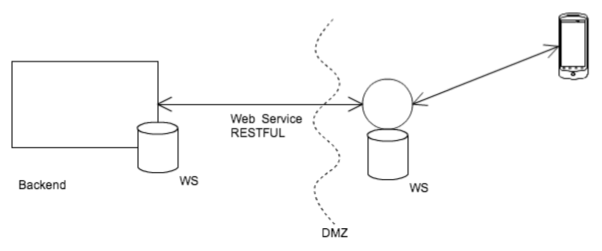
\includegraphics[width=10cm]{esquema_sistema_entrevista.png}
\caption{Esquema proporcionado por el analista durante la entrevista.}
\end{figure}
 
% Intervención del entrevistador
\paragraph{Diego} Se pregunta a Javier acerca del alcance que tiene dicho servicio, que limites de jurisdicción tiene dentro del término municipal.
 
% Intervención del responsable de operativa
\paragraph{Javier} Hay un limite de alcance, llega a la zona urbana y a la zona de núcleos rurales. No se limita sólo a zona urbana. Lo que ocurre es que para las zonas rurales hay un día a la semana. Las zonas rurales tienen su problemática aparte. Si no incluimos las zonas rurales, la puesta en producción va a ser más complicada. Nos recomienda hacer de las zonas rurales un sector más de las peticiones de servicio pero con la condición de que se les de sólo un día.  El motivo de que sólo se les de un día es debido a que las zonas rurales tienen una densidad de población más baja y la generación de residuos es más baja. Dentro de las zonas rurales, en el 99\% de los casos, hay una tipología de viviendas que permiten mantener el residuo una semana o dos al tratarse generalmente de parcelas grandes. Aunque en verano suele subir el número de peticiones de recogida en las zonas rurales, aunque sin cambiar la estructura funcional, esto es, sigue habiendo un solo día de recogida. Con un día de la semana, por el momento, suele ser suficiente.
 
% Intervención del entrevistador
\paragraph{Diego} Se pregunta acerca del número de peticiones por usuario en ubicaciones distintas.
 
% Intervención del responsable de operativa
\paragraph{Javier} Normalmente al día no se suele solicitar peticiones en diversas ubicaciones, nunca se ha dado el caso. Lo que si se suele dar es que haya mucho volumen de enseres y el mismo usuario solicite varias citas para el mismo punto de recogida, pero él personalmente nunca recuerda que se le hayan solicitado una petición por un usuario en diversos puntos.
 
% Intervención del analista
\paragraph{Enrique} Se nos recuerda que la aplicación debe desarrollarse en tres niveles
\begin{itemize}
\item Aplicación para dispositivo móvil (\textit{Android}).
\item  Servicio.
\item Aplicación simple de \textit{backend} para pruebas donde se muestre mediante una aplicación de escritorio simple la gestión de peticiones.
\end{itemize}
Inicialmente se hará una simulación de cómo funcionaría y posteriormente, cuando se lleve a producción el \text{backend}, será sustituido por el existente.
 
% Intervención del entrevistador
\paragraph{Diego} Se pregunta sobre la clasificación de zonas.
 
% Intervención del analista
\paragraph{Enrique} Dice que es muy simple y enumera las zonas : Centro, Río San Pedro, Las Canteras, Casines, Barrio Jarana, Meadero de la Reina y Zonas Rurales. Aunque en determinadas zonas, habiendo zonas rurales y urbanas, se distinguirían zonas de recogida ordinaria (diaria) y zonas de recogida especial (una vez a la semana). Se consideraría una primera versión y posteriormente, una versión de producción en la que se analice con más detenimiento la casuística.
 
 % Intervención del responsable de operativa
\paragraph{Javier} Sugiere que, en principio, para una primera versión quizás no sea tan importante dividir la localidad en 7 zonas sino en dos: zonas urbanas y zonas rurales. La casuística tampoco debe contemplar toda la casuística sino la que se contempla en el 90\% de los casos.

\paragraph{Diego}Finalmente se agradece su colaboración y se da por finalizada la entrevista. 


% Información de Licencia del documento
% This is set up to run with pdflatex.
%---------The file header---------------------------------------------
%---------------------------------------------------------------------
\chapter*{\rlap{GNU Free Documentation License}}
\phantomsection  % so hyperref creates bookmarks
\addcontentsline{toc}{chapter}{GNU Free Documentation License}
%\label{label_fdl}

 \begin{center}

       Version 1.3, 3 November 2008


 Copyright \copyright{} 2000, 2001, 2002, 2007, 2008  Free Software Foundation, Inc.
 
 \bigskip
 
     <http://fsf.org/>
  
 \bigskip
 
 Everyone is permitted to copy and distribute verbatim copies
 of this license document, but changing it is not allowed.
\end{center}


\begin{center}
{\bf\large Preamble}
\end{center}

The purpose of this License is to make a manual, textbook, or other
functional and useful document ``free'' in the sense of freedom: to
assure everyone the effective freedom to copy and redistribute it,
with or without modifying it, either commercially or noncommercially.
Secondarily, this License preserves for the author and publisher a way
to get credit for their work, while not being considered responsible
for modifications made by others.

This License is a kind of ``copyleft'', which means that derivative
works of the document must themselves be free in the same sense.  It
complements the GNU General Public License, which is a copyleft
license designed for free software.

We have designed this License in order to use it for manuals for free
software, because free software needs free documentation: a free
program should come with manuals providing the same freedoms that the
software does.  But this License is not limited to software manuals;
it can be used for any textual work, regardless of subject matter or
whether it is published as a printed book.  We recommend this License
principally for works whose purpose is instruction or reference.


\begin{center}
{\Large\bf 1. APPLICABILITY AND DEFINITIONS\par}
\phantomsection
\addcontentsline{toc}{section}{1. APPLICABILITY AND DEFINITIONS}
\end{center}

This License applies to any manual or other work, in any medium, that
contains a notice placed by the copyright holder saying it can be
distributed under the terms of this License.  Such a notice grants a
world-wide, royalty-free license, unlimited in duration, to use that
work under the conditions stated herein.  The ``\textbf{Document}'', below,
refers to any such manual or work.  Any member of the public is a
licensee, and is addressed as ``\textbf{you}''.  You accept the license if you
copy, modify or distribute the work in a way requiring permission
under copyright law.

A ``\textbf{Modified Version}'' of the Document means any work containing the
Document or a portion of it, either copied verbatim, or with
modifications and/or translated into another language.

A ``\textbf{Secondary Section}'' is a named appendix or a front-matter section of
the Document that deals exclusively with the relationship of the
publishers or authors of the Document to the Document's overall subject
(or to related matters) and contains nothing that could fall directly
within that overall subject.  (Thus, if the Document is in part a
textbook of mathematics, a Secondary Section may not explain any
mathematics.)  The relationship could be a matter of historical
connection with the subject or with related matters, or of legal,
commercial, philosophical, ethical or political position regarding
them.

The ``\textbf{Invariant Sections}'' are certain Secondary Sections whose titles
are designated, as being those of Invariant Sections, in the notice
that says that the Document is released under this License.  If a
section does not fit the above definition of Secondary then it is not
allowed to be designated as Invariant.  The Document may contain zero
Invariant Sections.  If the Document does not identify any Invariant
Sections then there are none.

The ``\textbf{Cover Texts}'' are certain short passages of text that are listed,
as Front-Cover Texts or Back-Cover Texts, in the notice that says that
the Document is released under this License.  A Front-Cover Text may
be at most 5 words, and a Back-Cover Text may be at most 25 words.

A ``\textbf{Transparent}'' copy of the Document means a machine-readable copy,
represented in a format whose specification is available to the
general public, that is suitable for revising the document
straightforwardly with generic text editors or (for images composed of
pixels) generic paint programs or (for drawings) some widely available
drawing editor, and that is suitable for input to text formatters or
for automatic translation to a variety of formats suitable for input
to text formatters.  A copy made in an otherwise Transparent file
format whose markup, or absence of markup, has been arranged to thwart
or discourage subsequent modification by readers is not Transparent.
An image format is not Transparent if used for any substantial amount
of text.  A copy that is not ``Transparent'' is called ``\textbf{Opaque}''.

Examples of suitable formats for Transparent copies include plain
ASCII without markup, Texinfo input format, LaTeX input format, SGML
or XML using a publicly available DTD, and standard-conforming simple
HTML, PostScript or PDF designed for human modification.  Examples of
transparent image formats include PNG, XCF and JPG.  Opaque formats
include proprietary formats that can be read and edited only by
proprietary word processors, SGML or XML for which the DTD and/or
processing tools are not generally available, and the
machine-generated HTML, PostScript or PDF produced by some word
processors for output purposes only.

The ``\textbf{Title Page}'' means, for a printed book, the title page itself,
plus such following pages as are needed to hold, legibly, the material
this License requires to appear in the title page.  For works in
formats which do not have any title page as such, ``Title Page'' means
the text near the most prominent appearance of the work's title,
preceding the beginning of the body of the text.

The ``\textbf{publisher}'' means any person or entity that distributes
copies of the Document to the public.

A section ``\textbf{Entitled XYZ}'' means a named subunit of the Document whose
title either is precisely XYZ or contains XYZ in parentheses following
text that translates XYZ in another language.  (Here XYZ stands for a
specific section name mentioned below, such as ``\textbf{Acknowledgements}'',
``\textbf{Dedications}'', ``\textbf{Endorsements}'', or ``\textbf{History}''.)  
To ``\textbf{Preserve the Title}''
of such a section when you modify the Document means that it remains a
section ``Entitled XYZ'' according to this definition.

The Document may include Warranty Disclaimers next to the notice which
states that this License applies to the Document.  These Warranty
Disclaimers are considered to be included by reference in this
License, but only as regards disclaiming warranties: any other
implication that these Warranty Disclaimers may have is void and has
no effect on the meaning of this License.


\begin{center}
{\Large\bf 2. VERBATIM COPYING\par}
\phantomsection
\addcontentsline{toc}{section}{2. VERBATIM COPYING}
\end{center}

You may copy and distribute the Document in any medium, either
commercially or noncommercially, provided that this License, the
copyright notices, and the license notice saying this License applies
to the Document are reproduced in all copies, and that you add no other
conditions whatsoever to those of this License.  You may not use
technical measures to obstruct or control the reading or further
copying of the copies you make or distribute.  However, you may accept
compensation in exchange for copies.  If you distribute a large enough
number of copies you must also follow the conditions in section~3.

You may also lend copies, under the same conditions stated above, and
you may publicly display copies.


\begin{center}
{\Large\bf 3. COPYING IN QUANTITY\par}
\phantomsection
\addcontentsline{toc}{section}{3. COPYING IN QUANTITY}
\end{center}


If you publish printed copies (or copies in media that commonly have
printed covers) of the Document, numbering more than 100, and the
Document's license notice requires Cover Texts, you must enclose the
copies in covers that carry, clearly and legibly, all these Cover
Texts: Front-Cover Texts on the front cover, and Back-Cover Texts on
the back cover.  Both covers must also clearly and legibly identify
you as the publisher of these copies.  The front cover must present
the full title with all words of the title equally prominent and
visible.  You may add other material on the covers in addition.
Copying with changes limited to the covers, as long as they preserve
the title of the Document and satisfy these conditions, can be treated
as verbatim copying in other respects.

If the required texts for either cover are too voluminous to fit
legibly, you should put the first ones listed (as many as fit
reasonably) on the actual cover, and continue the rest onto adjacent
pages.

If you publish or distribute Opaque copies of the Document numbering
more than 100, you must either include a machine-readable Transparent
copy along with each Opaque copy, or state in or with each Opaque copy
a computer-network location from which the general network-using
public has access to download using public-standard network protocols
a complete Transparent copy of the Document, free of added material.
If you use the latter option, you must take reasonably prudent steps,
when you begin distribution of Opaque copies in quantity, to ensure
that this Transparent copy will remain thus accessible at the stated
location until at least one year after the last time you distribute an
Opaque copy (directly or through your agents or retailers) of that
edition to the public.

It is requested, but not required, that you contact the authors of the
Document well before redistributing any large number of copies, to give
them a chance to provide you with an updated version of the Document.


\begin{center}
{\Large\bf 4. MODIFICATIONS\par}
\phantomsection
\addcontentsline{toc}{section}{4. MODIFICATIONS}
\end{center}

You may copy and distribute a Modified Version of the Document under
the conditions of sections 2 and 3 above, provided that you release
the Modified Version under precisely this License, with the Modified
Version filling the role of the Document, thus licensing distribution
and modification of the Modified Version to whoever possesses a copy
of it.  In addition, you must do these things in the Modified Version:

\begin{itemize}
\item[A.] 
   Use in the Title Page (and on the covers, if any) a title distinct
   from that of the Document, and from those of previous versions
   (which should, if there were any, be listed in the History section
   of the Document).  You may use the same title as a previous version
   if the original publisher of that version gives permission.
   
\item[B.]
   List on the Title Page, as authors, one or more persons or entities
   responsible for authorship of the modifications in the Modified
   Version, together with at least five of the principal authors of the
   Document (all of its principal authors, if it has fewer than five),
   unless they release you from this requirement.
   
\item[C.]
   State on the Title page the name of the publisher of the
   Modified Version, as the publisher.
   
\item[D.]
   Preserve all the copyright notices of the Document.
   
\item[E.]
   Add an appropriate copyright notice for your modifications
   adjacent to the other copyright notices.
   
\item[F.]
   Include, immediately after the copyright notices, a license notice
   giving the public permission to use the Modified Version under the
   terms of this License, in the form shown in the Addendum below.
   
\item[G.]
   Preserve in that license notice the full lists of Invariant Sections
   and required Cover Texts given in the Document's license notice.
   
\item[H.]
   Include an unaltered copy of this License.
   
\item[I.]
   Preserve the section Entitled ``History'', Preserve its Title, and add
   to it an item stating at least the title, year, new authors, and
   publisher of the Modified Version as given on the Title Page.  If
   there is no section Entitled ``History'' in the Document, create one
   stating the title, year, authors, and publisher of the Document as
   given on its Title Page, then add an item describing the Modified
   Version as stated in the previous sentence.
   
\item[J.]
   Preserve the network location, if any, given in the Document for
   public access to a Transparent copy of the Document, and likewise
   the network locations given in the Document for previous versions
   it was based on.  These may be placed in the ``History'' section.
   You may omit a network location for a work that was published at
   least four years before the Document itself, or if the original
   publisher of the version it refers to gives permission.
   
\item[K.]
   For any section Entitled ``Acknowledgements'' or ``Dedications'',
   Preserve the Title of the section, and preserve in the section all
   the substance and tone of each of the contributor acknowledgements
   and/or dedications given therein.
   
\item[L.]
   Preserve all the Invariant Sections of the Document,
   unaltered in their text and in their titles.  Section numbers
   or the equivalent are not considered part of the section titles.
   
\item[M.]
   Delete any section Entitled ``Endorsements''.  Such a section
   may not be included in the Modified Version.
   
\item[N.]
   Do not retitle any existing section to be Entitled ``Endorsements''
   or to conflict in title with any Invariant Section.
   
\item[O.]
   Preserve any Warranty Disclaimers.
\end{itemize}

If the Modified Version includes new front-matter sections or
appendices that qualify as Secondary Sections and contain no material
copied from the Document, you may at your option designate some or all
of these sections as invariant.  To do this, add their titles to the
list of Invariant Sections in the Modified Version's license notice.
These titles must be distinct from any other section titles.

You may add a section Entitled ``Endorsements'', provided it contains
nothing but endorsements of your Modified Version by various
parties---for example, statements of peer review or that the text has
been approved by an organization as the authoritative definition of a
standard.

You may add a passage of up to five words as a Front-Cover Text, and a
passage of up to 25 words as a Back-Cover Text, to the end of the list
of Cover Texts in the Modified Version.  Only one passage of
Front-Cover Text and one of Back-Cover Text may be added by (or
through arrangements made by) any one entity.  If the Document already
includes a cover text for the same cover, previously added by you or
by arrangement made by the same entity you are acting on behalf of,
you may not add another; but you may replace the old one, on explicit
permission from the previous publisher that added the old one.

The author(s) and publisher(s) of the Document do not by this License
give permission to use their names for publicity for or to assert or
imply endorsement of any Modified Version.


\begin{center}
{\Large\bf 5. COMBINING DOCUMENTS\par}
\phantomsection
\addcontentsline{toc}{section}{5. COMBINING DOCUMENTS}
\end{center}


You may combine the Document with other documents released under this
License, under the terms defined in section~4 above for modified
versions, provided that you include in the combination all of the
Invariant Sections of all of the original documents, unmodified, and
list them all as Invariant Sections of your combined work in its
license notice, and that you preserve all their Warranty Disclaimers.

The combined work need only contain one copy of this License, and
multiple identical Invariant Sections may be replaced with a single
copy.  If there are multiple Invariant Sections with the same name but
different contents, make the title of each such section unique by
adding at the end of it, in parentheses, the name of the original
author or publisher of that section if known, or else a unique number.
Make the same adjustment to the section titles in the list of
Invariant Sections in the license notice of the combined work.

In the combination, you must combine any sections Entitled ``History''
in the various original documents, forming one section Entitled
``History''; likewise combine any sections Entitled ``Acknowledgements'',
and any sections Entitled ``Dedications''.  You must delete all sections
Entitled ``Endorsements''.

\begin{center}
{\Large\bf 6. COLLECTIONS OF DOCUMENTS\par}
\phantomsection
\addcontentsline{toc}{section}{6. COLLECTIONS OF DOCUMENTS}
\end{center}

You may make a collection consisting of the Document and other documents
released under this License, and replace the individual copies of this
License in the various documents with a single copy that is included in
the collection, provided that you follow the rules of this License for
verbatim copying of each of the documents in all other respects.

You may extract a single document from such a collection, and distribute
it individually under this License, provided you insert a copy of this
License into the extracted document, and follow this License in all
other respects regarding verbatim copying of that document.


\begin{center}
{\Large\bf 7. AGGREGATION WITH INDEPENDENT WORKS\par}
\phantomsection
\addcontentsline{toc}{section}{7. AGGREGATION WITH INDEPENDENT WORKS}
\end{center}


A compilation of the Document or its derivatives with other separate
and independent documents or works, in or on a volume of a storage or
distribution medium, is called an ``aggregate'' if the copyright
resulting from the compilation is not used to limit the legal rights
of the compilation's users beyond what the individual works permit.
When the Document is included in an aggregate, this License does not
apply to the other works in the aggregate which are not themselves
derivative works of the Document.

If the Cover Text requirement of section~3 is applicable to these
copies of the Document, then if the Document is less than one half of
the entire aggregate, the Document's Cover Texts may be placed on
covers that bracket the Document within the aggregate, or the
electronic equivalent of covers if the Document is in electronic form.
Otherwise they must appear on printed covers that bracket the whole
aggregate.


\begin{center}
{\Large\bf 8. TRANSLATION\par}
\phantomsection
\addcontentsline{toc}{section}{8. TRANSLATION}
\end{center}


Translation is considered a kind of modification, so you may
distribute translations of the Document under the terms of section~4.
Replacing Invariant Sections with translations requires special
permission from their copyright holders, but you may include
translations of some or all Invariant Sections in addition to the
original versions of these Invariant Sections.  You may include a
translation of this License, and all the license notices in the
Document, and any Warranty Disclaimers, provided that you also include
the original English version of this License and the original versions
of those notices and disclaimers.  In case of a disagreement between
the translation and the original version of this License or a notice
or disclaimer, the original version will prevail.

If a section in the Document is Entitled ``Acknowledgements'',
``Dedications'', or ``History'', the requirement (section~4) to Preserve
its Title (section~1) will typically require changing the actual
title.


\begin{center}
{\Large\bf 9. TERMINATION\par}
\phantomsection
\addcontentsline{toc}{section}{9. TERMINATION}
\end{center}


You may not copy, modify, sublicense, or distribute the Document
except as expressly provided under this License.  Any attempt
otherwise to copy, modify, sublicense, or distribute it is void, and
will automatically terminate your rights under this License.

However, if you cease all violation of this License, then your license
from a particular copyright holder is reinstated (a) provisionally,
unless and until the copyright holder explicitly and finally
terminates your license, and (b) permanently, if the copyright holder
fails to notify you of the violation by some reasonable means prior to
60 days after the cessation.

Moreover, your license from a particular copyright holder is
reinstated permanently if the copyright holder notifies you of the
violation by some reasonable means, this is the first time you have
received notice of violation of this License (for any work) from that
copyright holder, and you cure the violation prior to 30 days after
your receipt of the notice.

Termination of your rights under this section does not terminate the
licenses of parties who have received copies or rights from you under
this License.  If your rights have been terminated and not permanently
reinstated, receipt of a copy of some or all of the same material does
not give you any rights to use it.


\begin{center}
{\Large\bf 10. FUTURE REVISIONS OF THIS LICENSE\par}
\phantomsection
\addcontentsline{toc}{section}{10. FUTURE REVISIONS OF THIS LICENSE}
\end{center}


The Free Software Foundation may publish new, revised versions
of the GNU Free Documentation License from time to time.  Such new
versions will be similar in spirit to the present version, but may
differ in detail to address new problems or concerns.  See
http://www.gnu.org/copyleft/.

Each version of the License is given a distinguishing version number.
If the Document specifies that a particular numbered version of this
License ``or any later version'' applies to it, you have the option of
following the terms and conditions either of that specified version or
of any later version that has been published (not as a draft) by the
Free Software Foundation.  If the Document does not specify a version
number of this License, you may choose any version ever published (not
as a draft) by the Free Software Foundation.  If the Document
specifies that a proxy can decide which future versions of this
License can be used, that proxy's public statement of acceptance of a
version permanently authorizes you to choose that version for the
Document.


\begin{center}
{\Large\bf 11. RELICENSING\par}
\phantomsection
\addcontentsline{toc}{section}{11. RELICENSING}
\end{center}


``Massive Multiauthor Collaboration Site'' (or ``MMC Site'') means any
World Wide Web server that publishes copyrightable works and also
provides prominent facilities for anybody to edit those works.  A
public wiki that anybody can edit is an example of such a server.  A
``Massive Multiauthor Collaboration'' (or ``MMC'') contained in the
site means any set of copyrightable works thus published on the MMC
site.

``CC-BY-SA'' means the Creative Commons Attribution-Share Alike 3.0
license published by Creative Commons Corporation, a not-for-profit
corporation with a principal place of business in San Francisco,
California, as well as future copyleft versions of that license
published by that same organization.

``Incorporate'' means to publish or republish a Document, in whole or
in part, as part of another Document.

An MMC is ``eligible for relicensing'' if it is licensed under this
License, and if all works that were first published under this License
somewhere other than this MMC, and subsequently incorporated in whole
or in part into the MMC, (1) had no cover texts or invariant sections,
and (2) were thus incorporated prior to November 1, 2008.

The operator of an MMC Site may republish an MMC contained in the site
under CC-BY-SA on the same site at any time before August 1, 2009,
provided the MMC is eligible for relicensing.


\begin{center}
{\Large\bf ADDENDUM: How to use this License for your documents\par}
\phantomsection
\addcontentsline{toc}{section}{ADDENDUM: How to use this License for your documents}
\end{center}

To use this License in a document you have written, include a copy of
the License in the document and put the following copyright and
license notices just after the title page:

\bigskip
\begin{quote}
    Copyright \copyright{}  YEAR  YOUR NAME.
    Permission is granted to copy, distribute and/or modify this document
    under the terms of the GNU Free Documentation License, Version 1.3
    or any later version published by the Free Software Foundation;
    with no Invariant Sections, no Front-Cover Texts, and no Back-Cover Texts.
    A copy of the license is included in the section entitled ``GNU
    Free Documentation License''.
\end{quote}
\bigskip
    
If you have Invariant Sections, Front-Cover Texts and Back-Cover Texts,
replace the ``with \dots\ Texts.'' line with this:

\bigskip
\begin{quote}
    with the Invariant Sections being LIST THEIR TITLES, with the
    Front-Cover Texts being LIST, and with the Back-Cover Texts being LIST.
\end{quote}
\bigskip
    
If you have Invariant Sections without Cover Texts, or some other
combination of the three, merge those two alternatives to suit the
situation.

If your document contains nontrivial examples of program code, we
recommend releasing these examples in parallel under your choice of
free software license, such as the GNU General Public License,
to permit their use in free software.

%---------------------------------------------------------------------


\end{document}
